\chapter{Initial experiments}\label{chap:exp}

\section{Preprocessing experiment}
In this experiment about preprocessing, we mainly use the library OpenCV to provide the results for each techniques mentioned in Chapter \ref{background} and give an evaluation for the experiment result. \\
In this section, we are going through each steps in the process. We also have some pictures to make it clearer about the result of each step. The original image we used in this section is captured in a good environment condition.
\subsection{Convert RGB image to grayscale image}
The first step of all is convert a RGB image into grayscale image. This is a simple to remove the color part from the captured image. In this step, we use luminosity method and the result can see in the \ref{fig:grayscaleImage}:

\begin{figure}[h]
\centering
    \begin{subfigure}{0.4\textwidth}
        \centering
        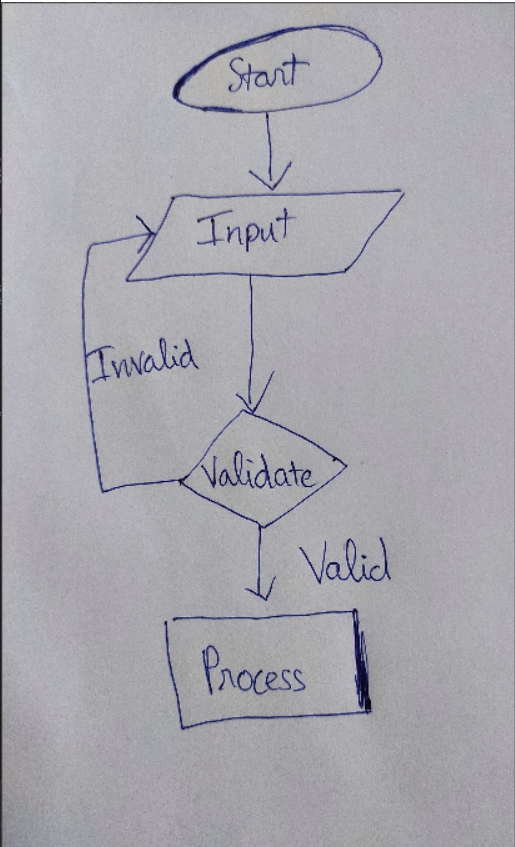
\includegraphics[width=5cm, height=6.5cm]{Images/Preprocessing/rawImage.png}
        \caption{Original Image}
        \label{fig:rawImage}
    \end{subfigure}
    \begin{subfigure}{0.4\textwidth}
        \centering
        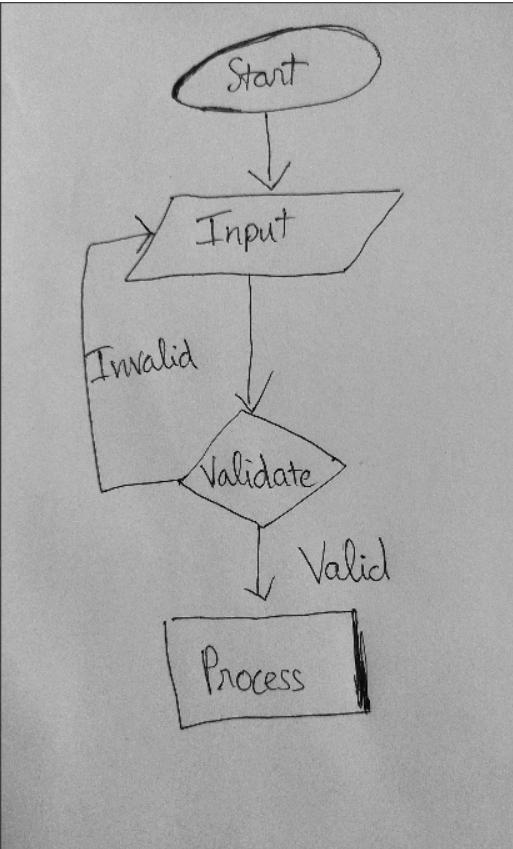
\includegraphics[width=5cm, height=6.5cm]{Images/Preprocessing/grayscale.png}
        \caption{Grayscale image}
        \label{fig:grayscaleImage}
    \end{subfigure}
    \caption{Figure \ref{fig:rawImage} is the original handwriting flow chart; figure \ref{fig:grayscaleImage} is grayscale version of the figure \ref{fig:rawImage}} 
    \label{fig:grayscale_step}
\end{figure}

\subsection{Histogram equalization}
\hspace{0.5cm} {In this step, we use Histogram Equalization technique to improve contrasts in the grayscale image.}

\begin{figure}[h]
    \centering
    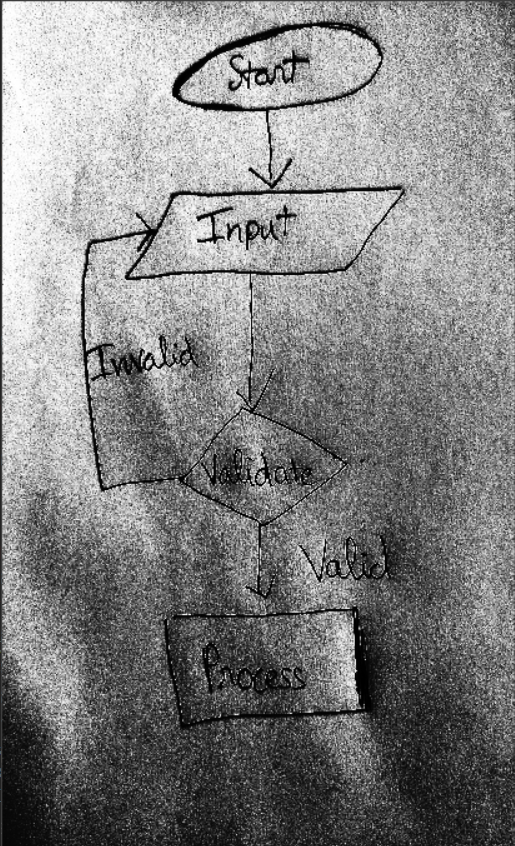
\includegraphics[width=5cm,height=6.5cm]{Images/Preprocessing/histoequal.png}
    \caption{Histogram equalized image converted from figure \ref{fig:grayscaleImage}}
    \label{fig:histoEqualized}
\end{figure}

\begin{figure}[h]
\centering
    \begin{subfigure}{0.4\textwidth}
        \centering
        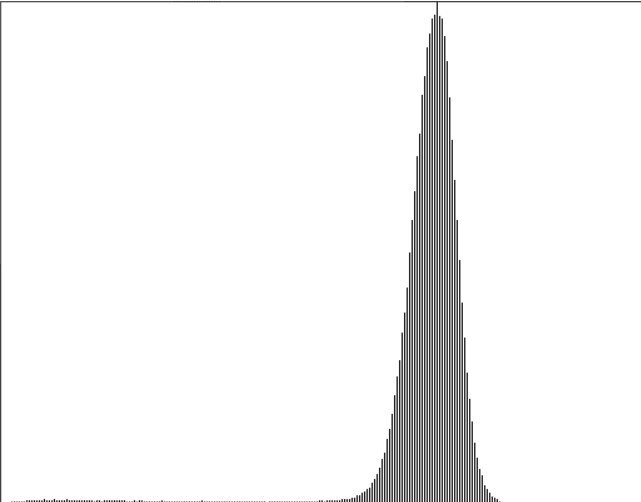
\includegraphics[width=5cm,height=7cm]{Images/Preprocessing/grayhisto.png}
        \caption{Original Histogram}
        \label{fig:origin_histogram}
    \end{subfigure}
    \begin{subfigure}{0.4\textwidth}
        \centering
        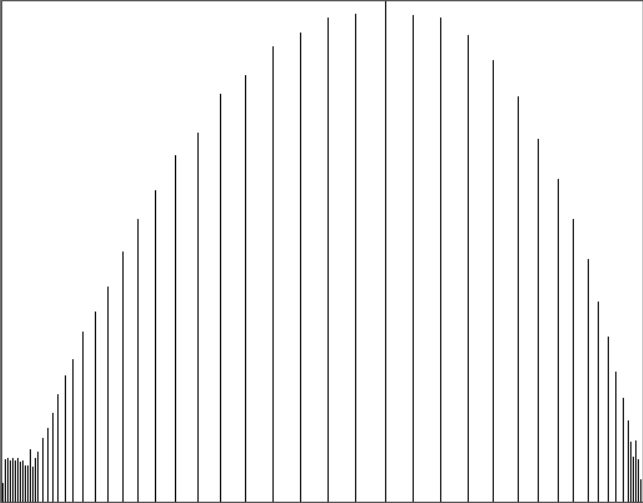
\includegraphics[width=5cm,height=7cm]{Images/Preprocessing/equalhisto.png}
        \caption{Equalized histogram}
        \label{fig:Equalizedhistogram}
    \end{subfigure}
    \caption{Figure \ref{fig:origin_histogram} is the histogram of figure \ref{fig:grayscaleImage}; figure \ref{fig:Equalizedhistogram} } is the figure \ref{fig:origin_histogram} converted to by using Histogram Equalization
    \label{fig:histogram_equalization}
\end{figure}

Observe the figure \ref{fig:histoEqualized}, we can see that this procedure make the image worse than the figure \ref{fig:grayscaleImage}. From the result, we decided to remove the step Histogram Equalization from preprocessing.
\subsection{Image smoothing}
\begin{figure}[h]
    \centering
    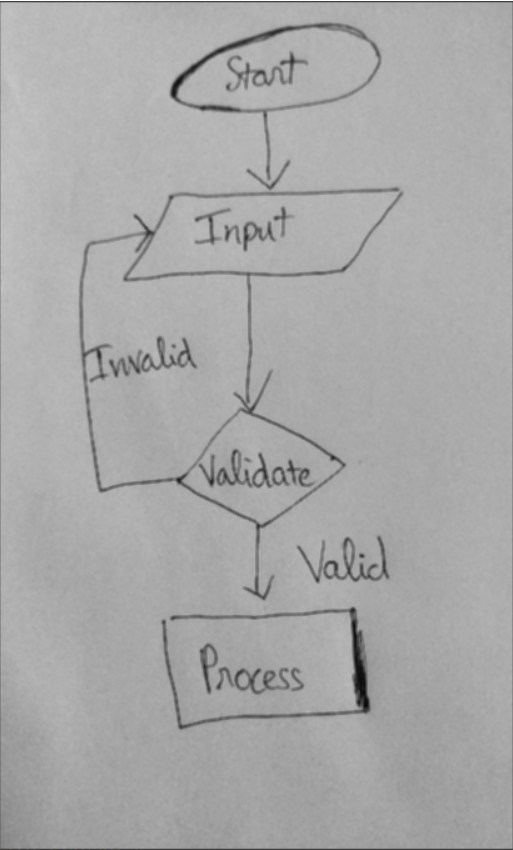
\includegraphics[width=5cm,height=7cm]{Images/Preprocessing/gaussian.png}
    \caption{Gaussian blur applies on \ref{fig:grayscaleImage}}
    \label{fig:gaussian_blur}
\end{figure}
In this step, we filter the noise from the image. As we can see from the figure 6.1 (b), the noise in the figure is Gaussian noise, which represents statistical noise having probability density function equal to the normal distribution, which is also known as the Gaussian distribution. Therefore, to remove this type of noise, Gaussian filter is used in this case. The blurred image after using Gaussian filter is in figure \ref{fig:gaussian_blur}.

\subsection{Convert into binary image}
\begin{figure}[t]
\centering
    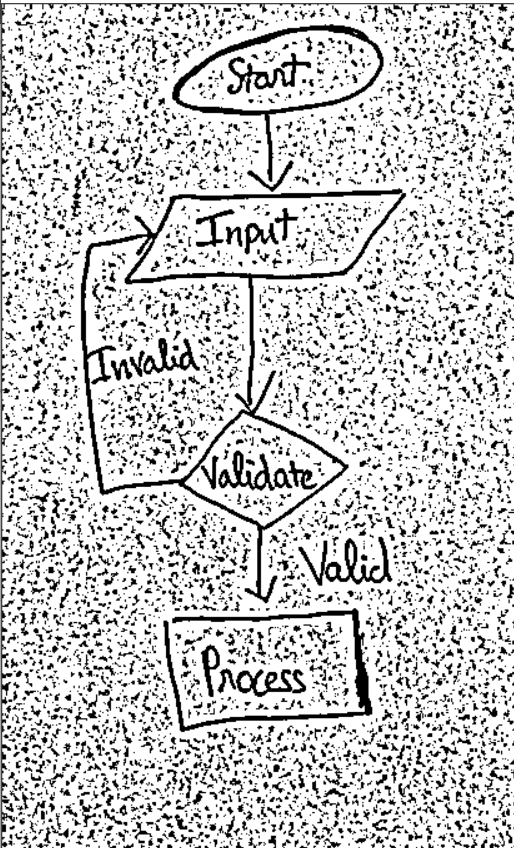
\includegraphics[scale=0.35]{Images/Preprocessing/binaryimage.png}
    \caption{Binary image}
    \label{fig: binary_image}
\end{figure}

In this step, we use the Adaptive Thresholding technique to binarize figure \ref{fig:gaussian_blur}. The result of this step is in figure 6.5. In addition, we also show the result of converting the histogram equalization image, which also is blurred by Gaussian blur, into binary image in this figure. \\

From figure \ref{fig: binary_image}, it can be seen that there are speckle noises which is needed to be removed.

\subsection{Speckle filter}

\begin{figure}[t]
    \centering
    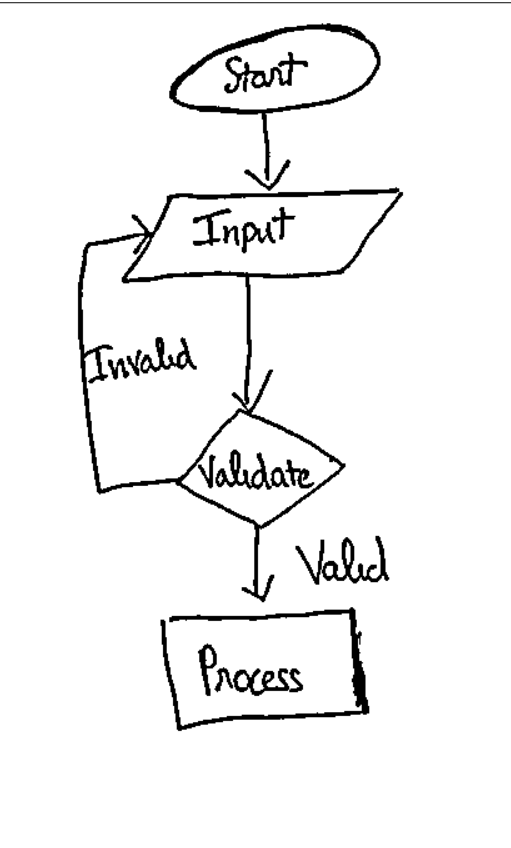
\includegraphics[scale=0.35]{Images/Preprocessing/clearBI.png}
    \caption{Filter speckles in binary image}
    \label{fig:specfilter_BI}
\end{figure}

This is the final step of preprocessing. In this step, we use the filterSpeckles() function from OpenCV to remove the blobs in the binary image. The result we get is in figure \ref{fig:specfilter_BI}.

This function gives a good result with the figure \ref{fig:specfilter_BI}, which separates the flowchart with the black color from the white background.

\section{Web server communication}
This system is designed to transfer images taken from client devices and send them to the web server to process. However, most of the current mobile device has a great camera quality which can produce high definition pictures but also has a large size. Trying to transfer the whole file in one request may cause disruption and corruption of the file. However, the Hypertext Transfer Protocol (HTTP) supports a Multi part Request, which is a combination of one or more sets of data into a single body. The body is then divided into many ''body parts'', each of them has an encapsulation boundary ahead in the combination and the last one is enclosed with a closing boundary \cite{58}. The content-type ''multipart/form-data'' allows the app to send the image by blocks of data, which will then be collected by the web server.

Flutter HTTP package supports multipart/form-data requests. When this request is called, it automatically sets the Content-Type header to multipart/form-data. This value will override any value set by the user. There are many ways to perform this request, in this experiment, we used MultipartFile.fromBytes, which will create a new multi part file from a byte array. That means first the image needs to be converted into a list of bytes, then will be transformed into a multipart file and send over (see Figure \ref{fig:ImageSendClient}). The web server will receive the file as a stream (see Figure \ref{fig:ImageSendServer}).

\begin{figure}[!b]
\centering
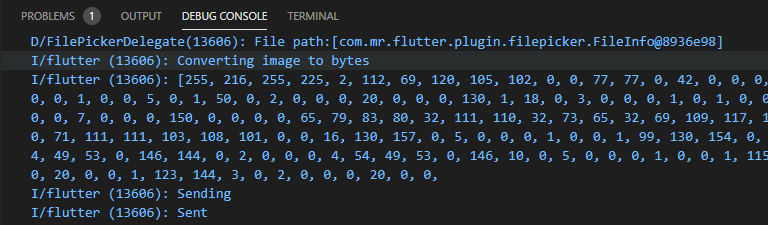
\includegraphics[width=14cm]{Images/App/ImageSendClient.png}
\caption{Client application sending image log}
\label{fig:ImageSendClient}

\centering
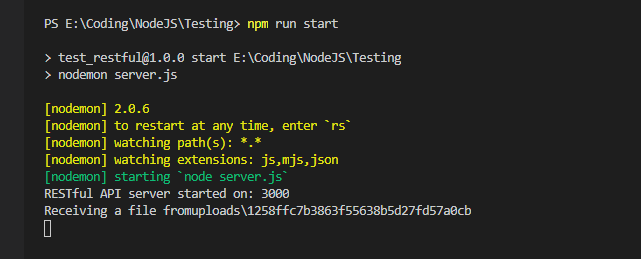
\includegraphics[width=14cm]{Images/App/ImageSendServer.png}
\caption{Server log}
\label{fig:ImageSendServer}
\end{figure}

\section{Display diagram on device}
\subsection{Interactive Viewer and Matrix4}
In order to handle user action like panning, zooming and moving around the diagram, the surface that used to draw the diagram on need to be interactive. One of the most powerful widget (all components in Flutter is fundamentally defined as a widget) in Flutter is the transform class widget which is able to change the perspective of the user of a widget. Basically it makes changes in how the widget look and behave so that developer can create new and more complex component from the existed one. It is controlled by a four dimensions matrix that define how the widget will transform called ''matrix4''. While Flutter also provides other easier ways for scaling, rotating and translating, ''matrix4'' allows more customization. ''Interactive Viewer'' is one of the widget created from the transform class that allows user to transform all the components inside by dragging to pan or pinching to zoom. The difference of it from the rest is it can create a wide space for interacting and is mainly used to grab the widgets that is too big to fit inside the screen, which is a perfect space to draw the diagram on. ''Interactive Viewer'' transforms itself by changing some specific value in the ''matrix4''.

For example, in the table \ref{fig:matrix4}, we can see a 4x4 matrix represent the ''matrix4'', by default it is an identity matrix (which has all the value in the diagonal line equal to 1). In that state, the widget is in its normal size (see Figure \ref{fig:defaultspace}). Then it can  be tweeted in order to achieve the prefer shape.

To scale the widget (change its size to make it bigger or smaller): we can change the value ''a'' and ''b'' in the table \ref{fig:matrix4} into a value greater than zero (zero value will make the matrix unable to reverted ). Value smaller than one will make it shrink and value greater than one will expand it in the corresponding dimension. In the table, value ''a'' controls the X-dimension or the width of the space (see Figure \ref{fig:xscale}) and ''b'' does the same for the height (Y-dimension) (see Figure \ref{fig:yscale}).

In a two dimension perspective, that maybe enough to express most of the form of the space. However, there is also the value ''c'' that may influence the way user interact with the space, which scaling in the Z-dimension. For instance, in Figure \ref{fig:zscaledemo}, value ''c'' in position 3,3 has been changed to 2.0 but the space remain unchanged. In theory, the Z-dimension represents how deep the widget should look like, then it may seem to be unnecessary in a 2D space, but as it is zoomed out (see Figure \ref{fig:zoomzscale}) then the zooming scale has been increased, as if the widget is now further from the screen perspective.

Finally, The space can be moved the space around in X and Y dimension by changing value in ''d'' (4,1) and ''e'' (4,2) position. Value in this position will be consider as the amount of pixels that the space move. For example, in Figure \ref{fig:xmove}, ''d'' is set to 100, that means the space will move right 100 pixels. The same thing with Figure  \ref{fig:ymove} with ''e'' equals 100, the space will move down 100 pixels.

\subsection{Result}
After applying the previous widget and display the symbol and line with a stack in the diagram space, we get the result as show in figure \ref{fig:result}.


\begin{figure}[t]
    \centering
    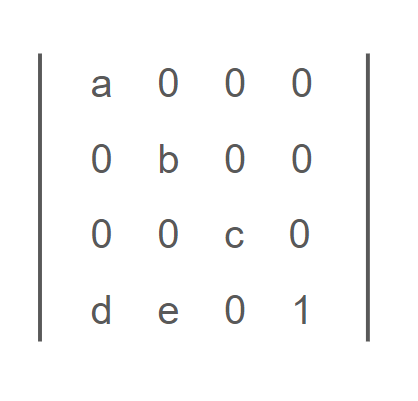
\includegraphics[width=8cm]{Images/App/matrix4.png}
    \caption{Example of matrix4}
    \label{fig:matrix4}
\end{figure}

\begin{figure}[b]
    \begin{subfigure}{0.4\textwidth}
        \centering
        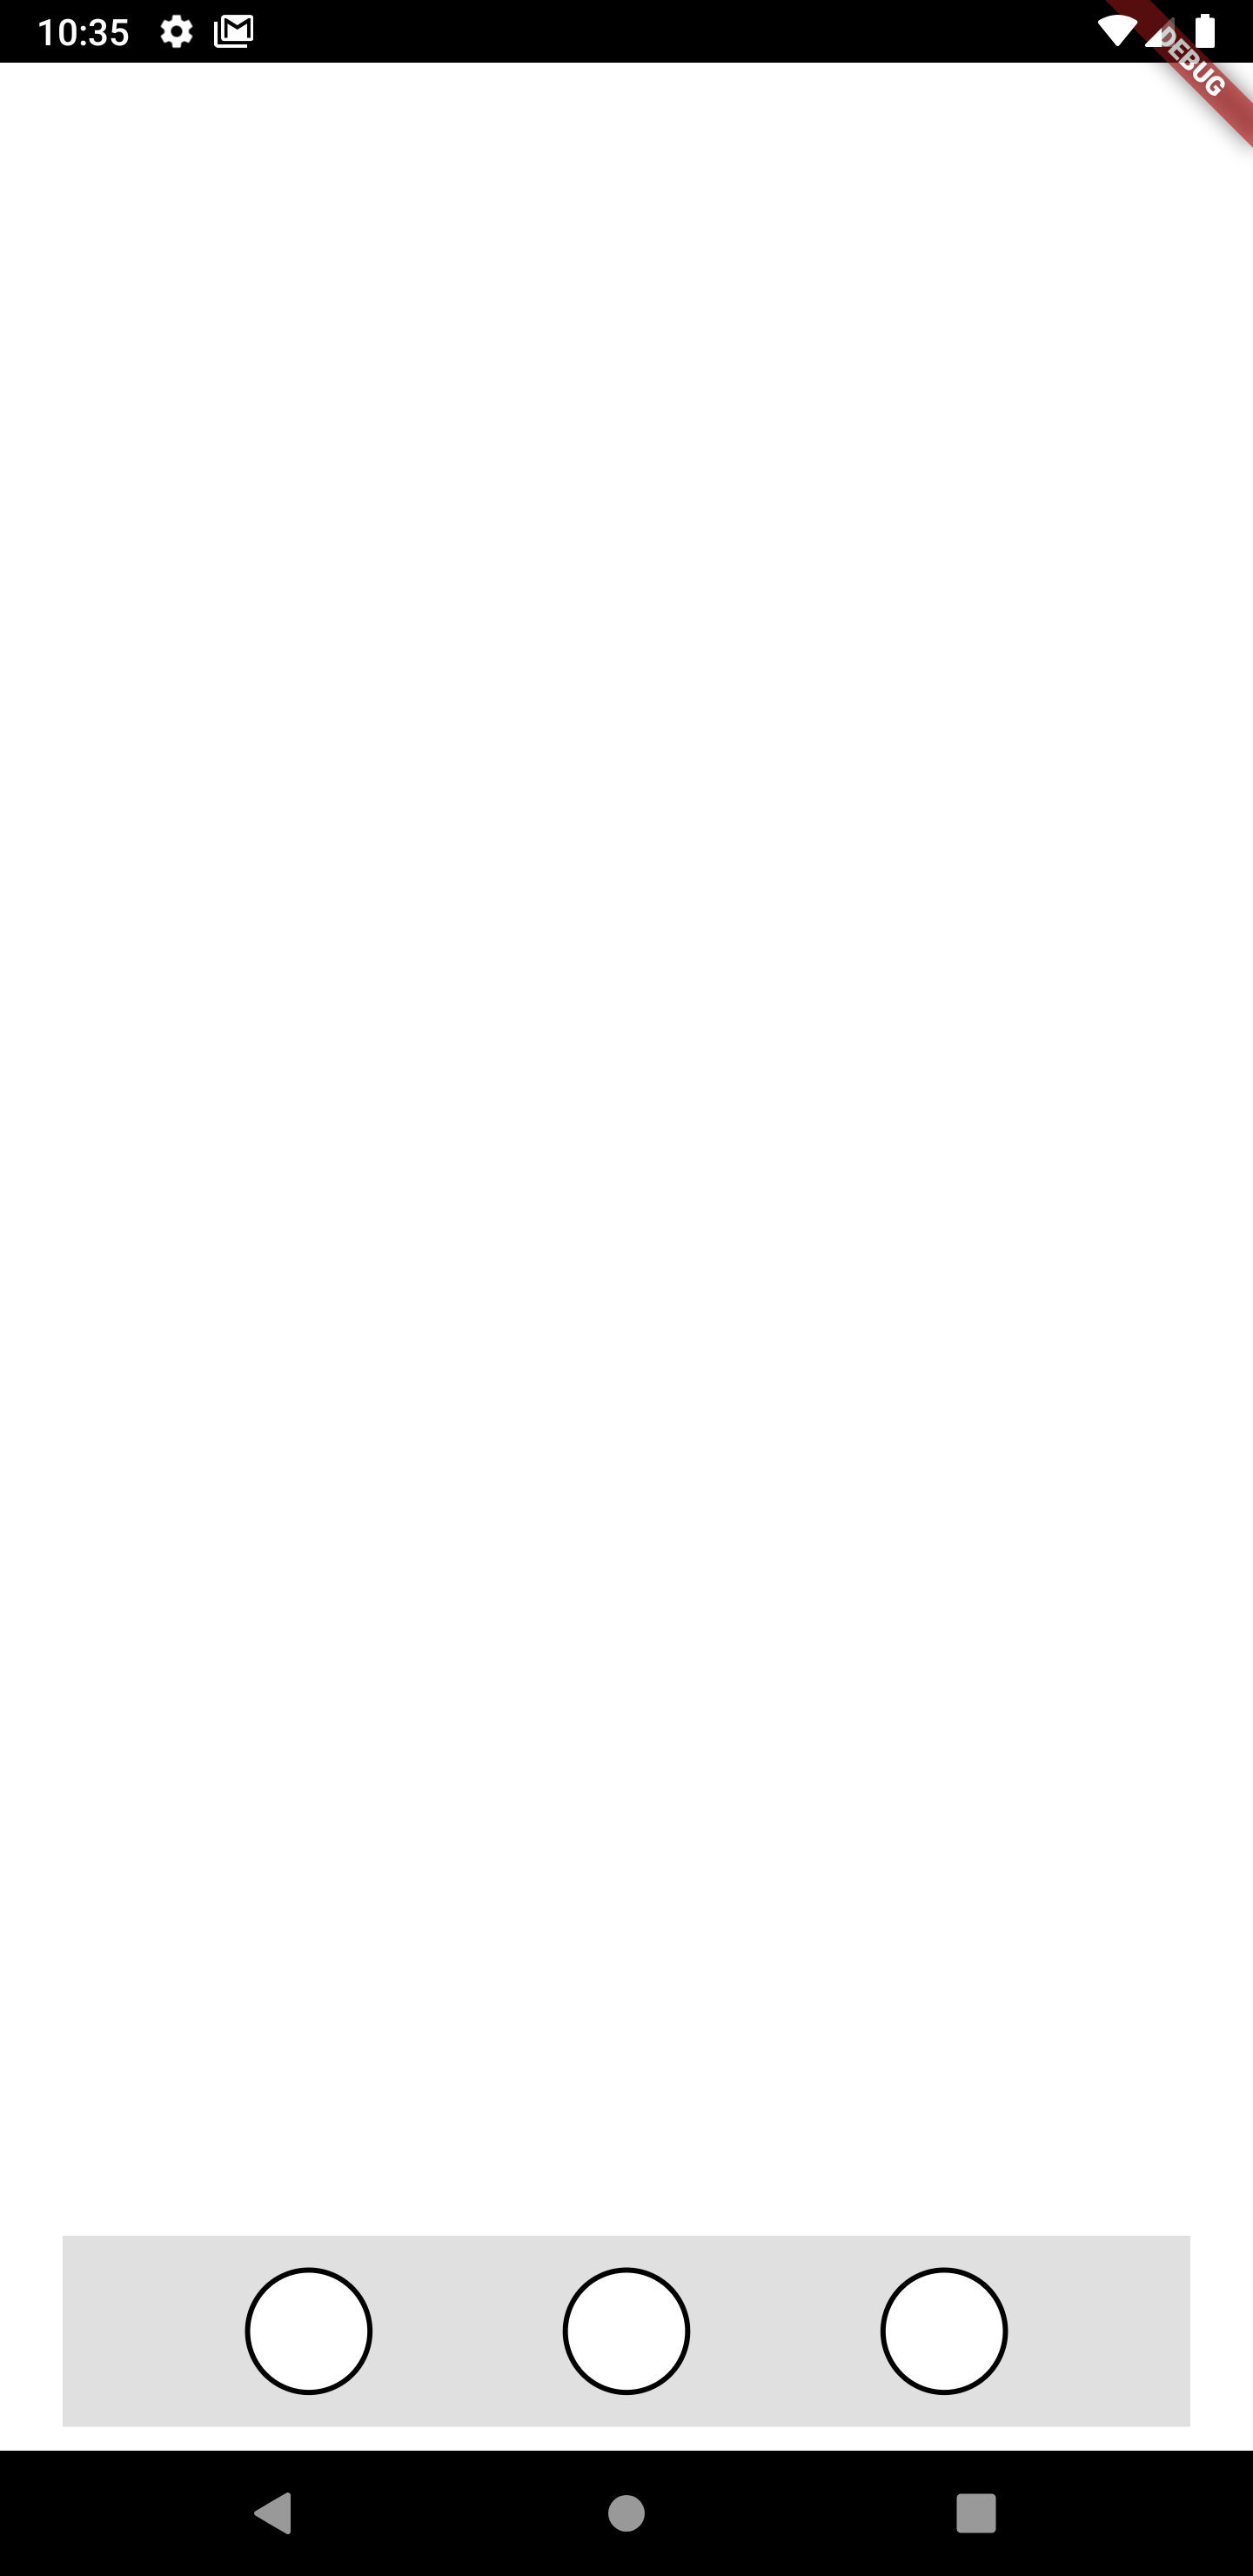
\includegraphics[width=5cm]{Images/App/fullspace.png}
        \caption{Default}
        \label{fig:fullspace}
    \end{subfigure}
    \hfill
    \begin{subfigure}{0.4\textwidth}
        \centering
        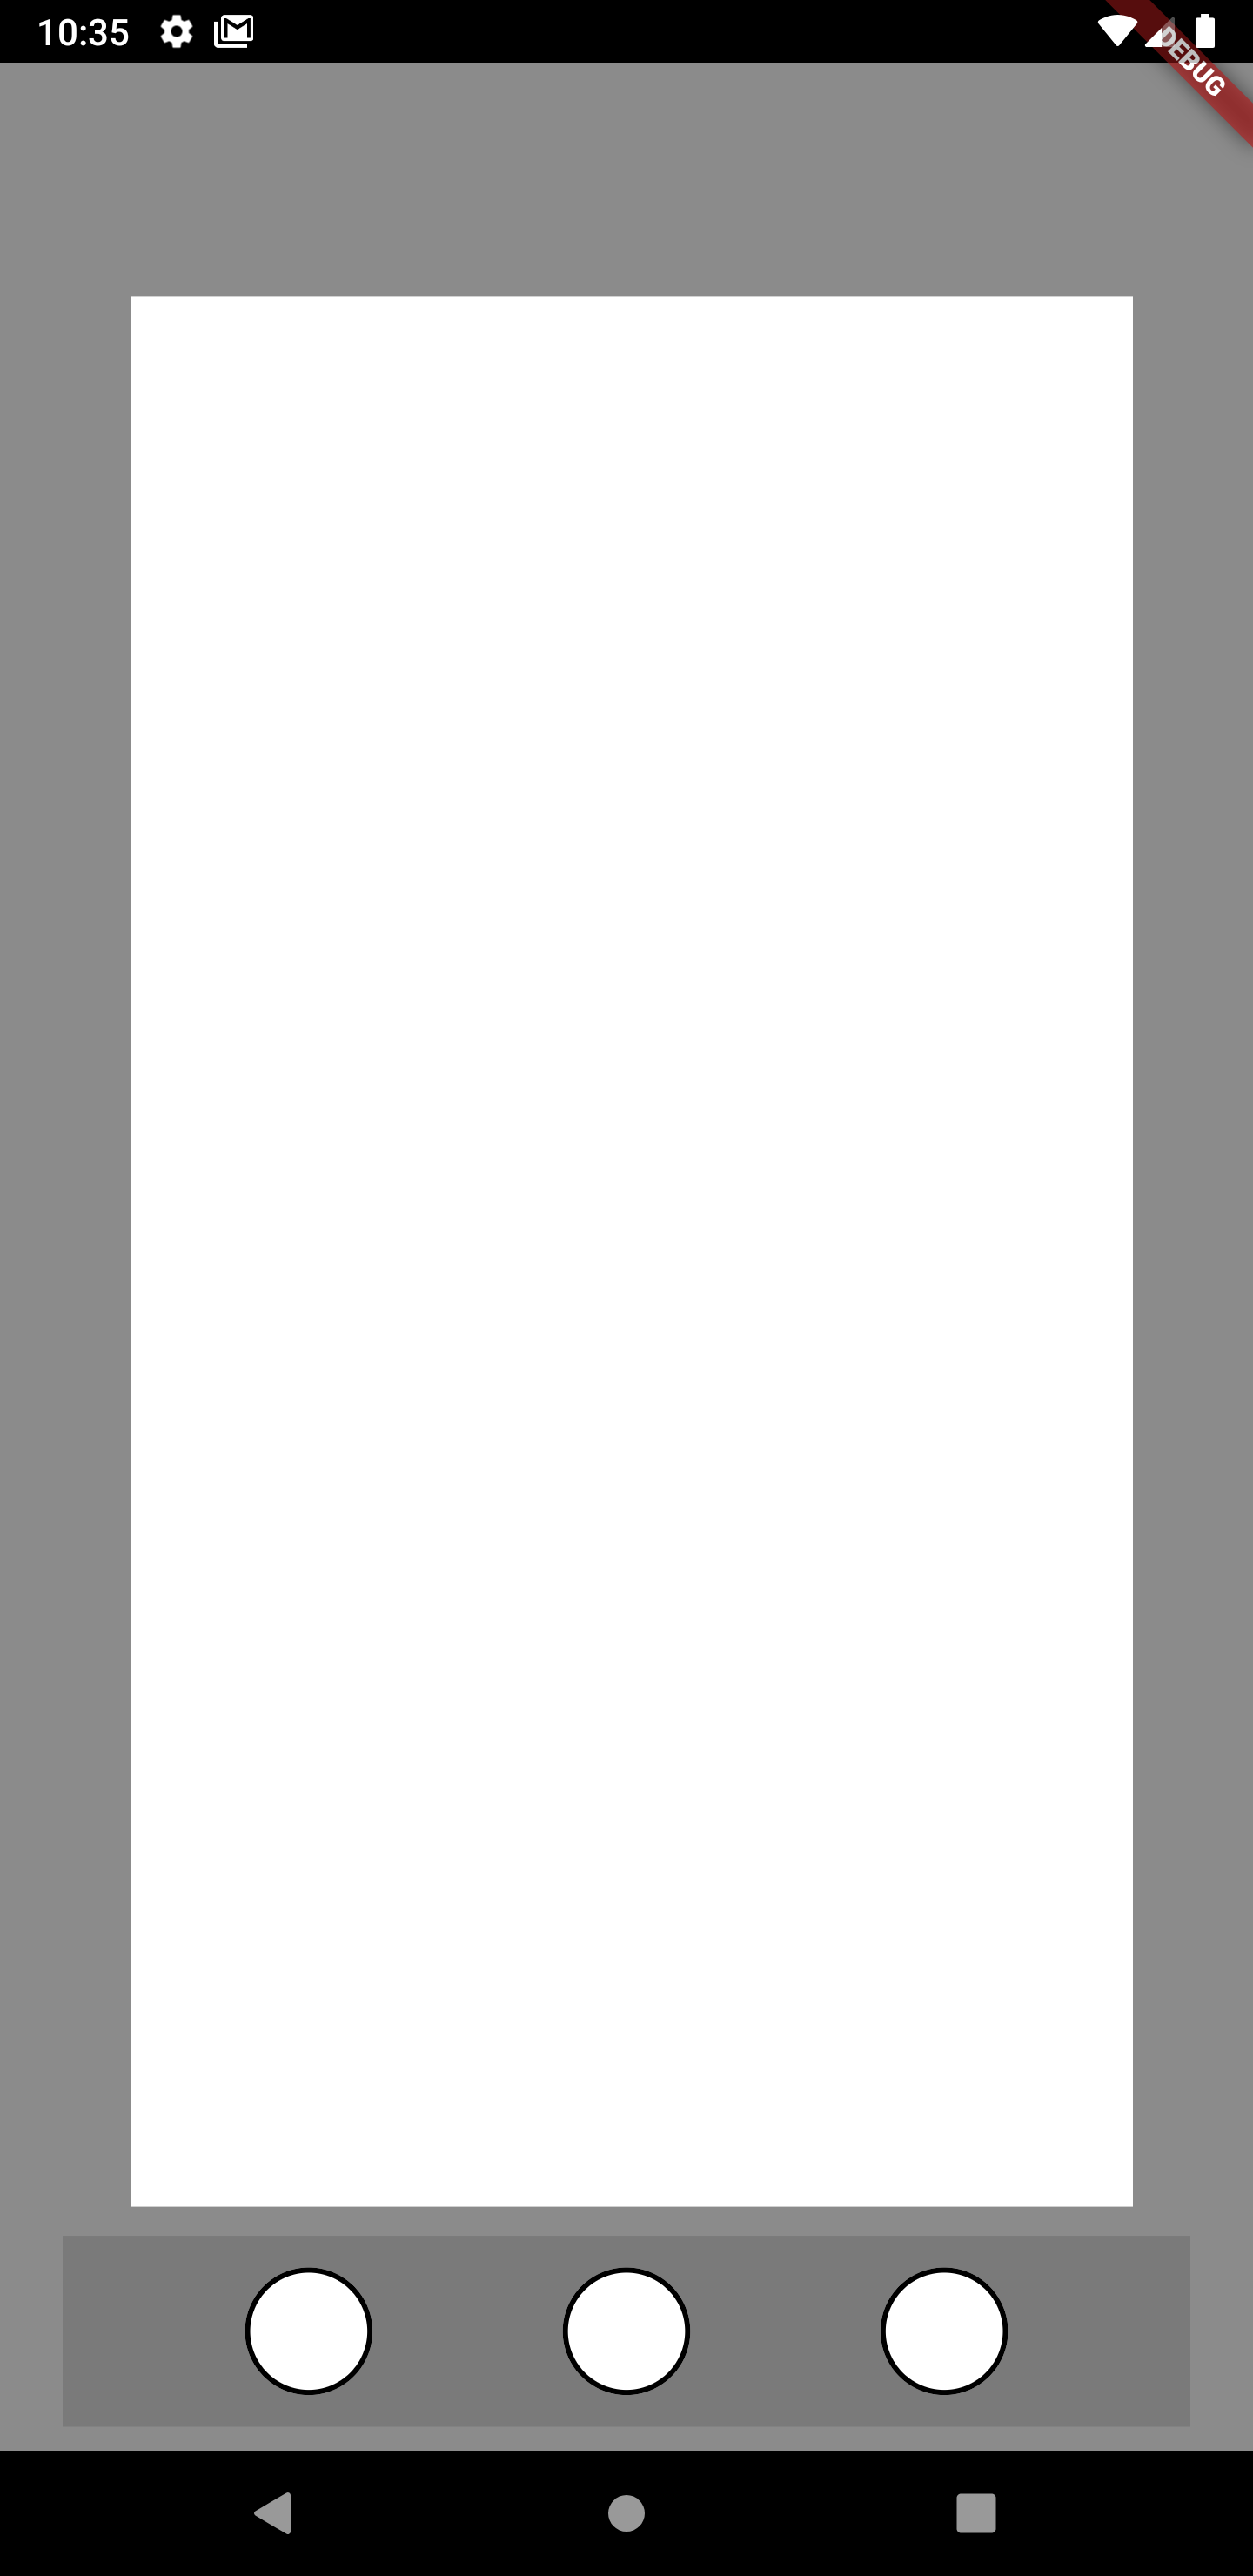
\includegraphics[width=5cm]{Images/App/fullzoom.png}
        \caption{Zoom out from the default}
        \label{fig:fullzoom}
    \end{subfigure}
    \caption{Interactive space using identity matrix}
    \label{fig:defaultspace}
\end{figure}

\begin{figure}[b]
    \begin{subfigure}{0.4\textwidth}
        \centering
        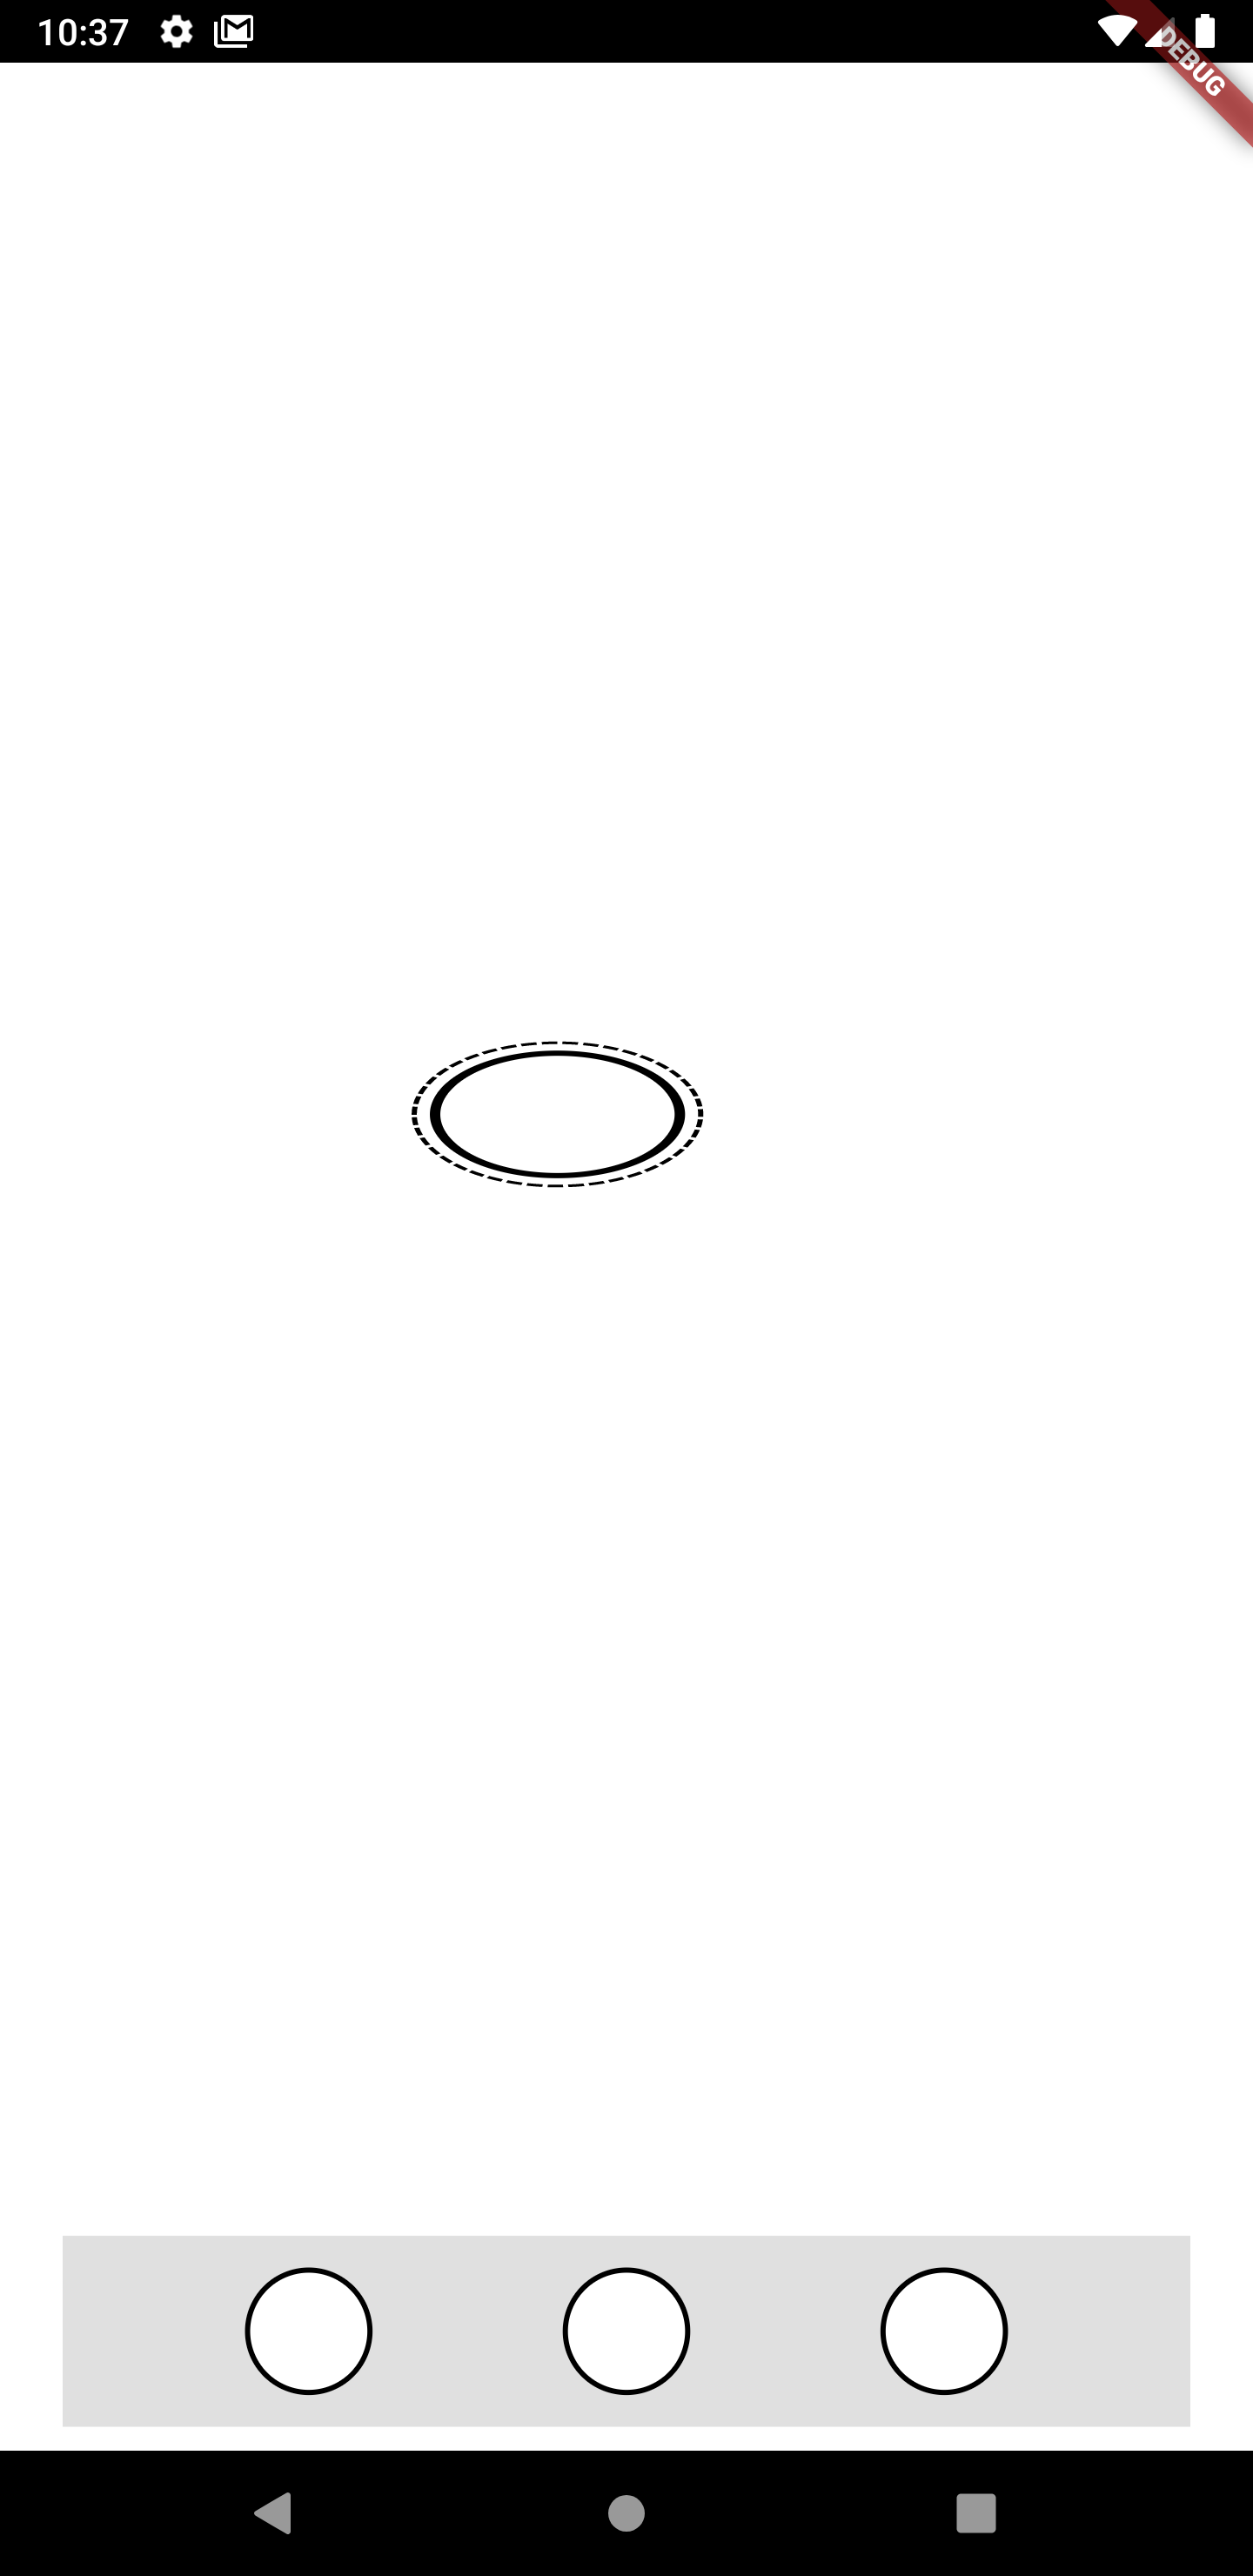
\includegraphics[width=5cm]{Images/App/xscale.png}
        \caption{Value a (1,1) = 2.0}
        \label{fig:xscale}
    \end{subfigure}
    \hfill
    \begin{subfigure}{0.4\textwidth}
        \centering
        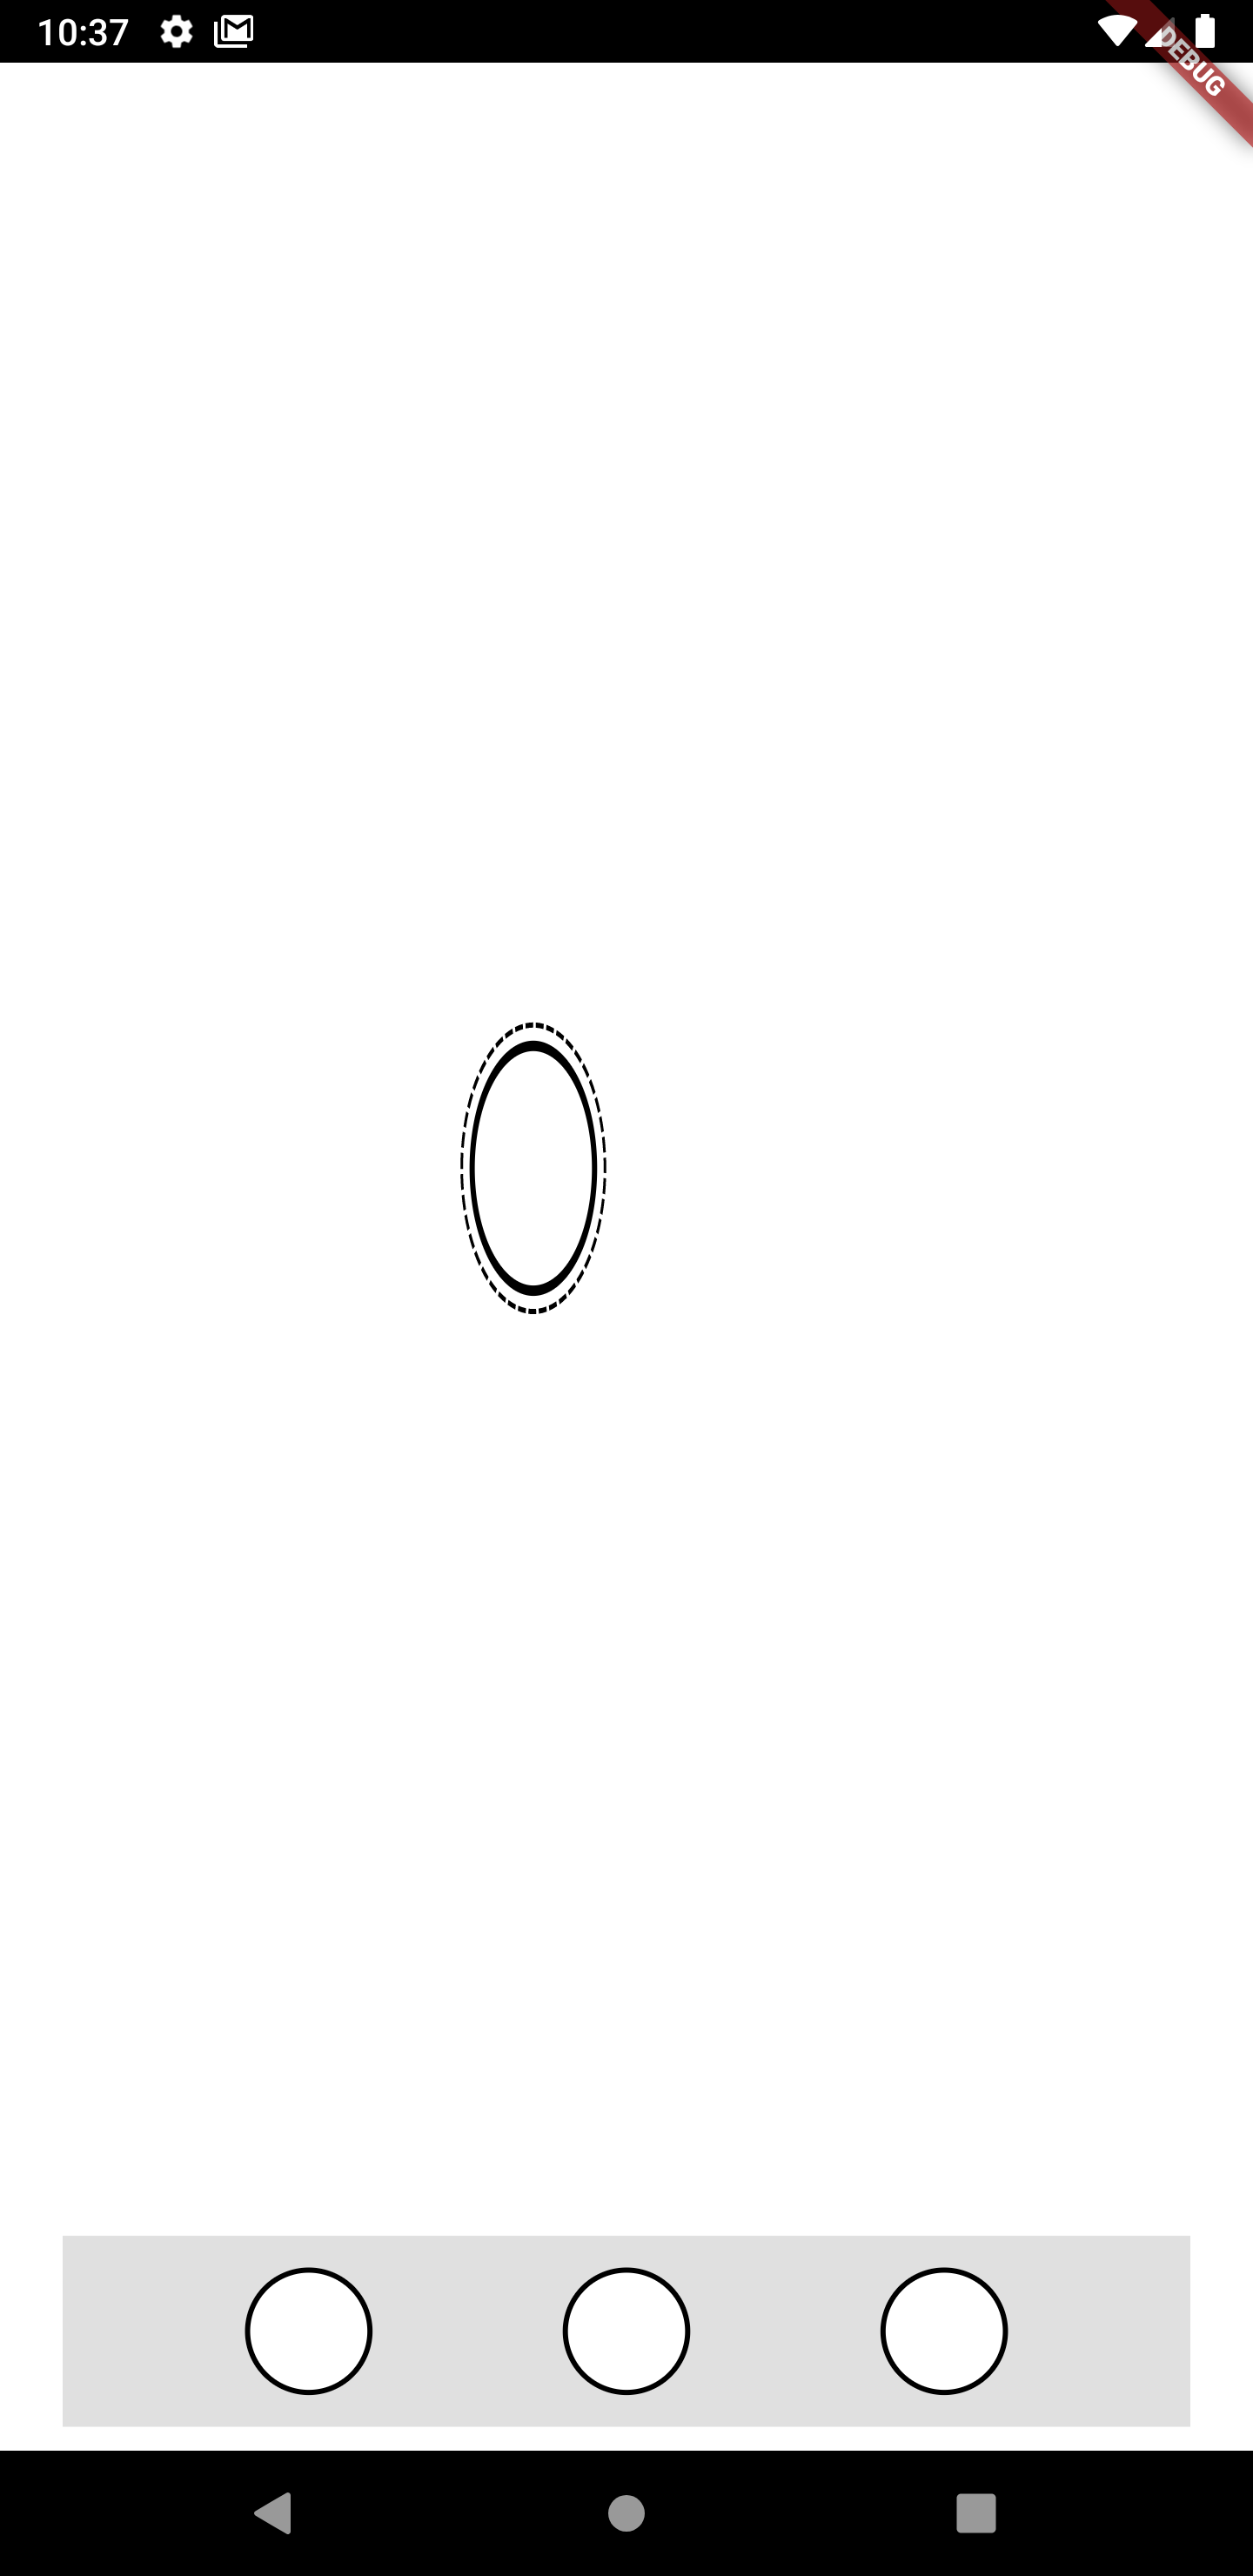
\includegraphics[width=5cm]{Images/App/yscale.png}
        \caption{Value b (2,2) = 2.0}
        \label{fig:yscale}
    \end{subfigure}
    \caption{Scaling in X and Y}
    \label{fig:xysacle}
\end{figure}

\begin{figure}[b]
    \begin{subfigure}{0.4\textwidth}
        \centering
        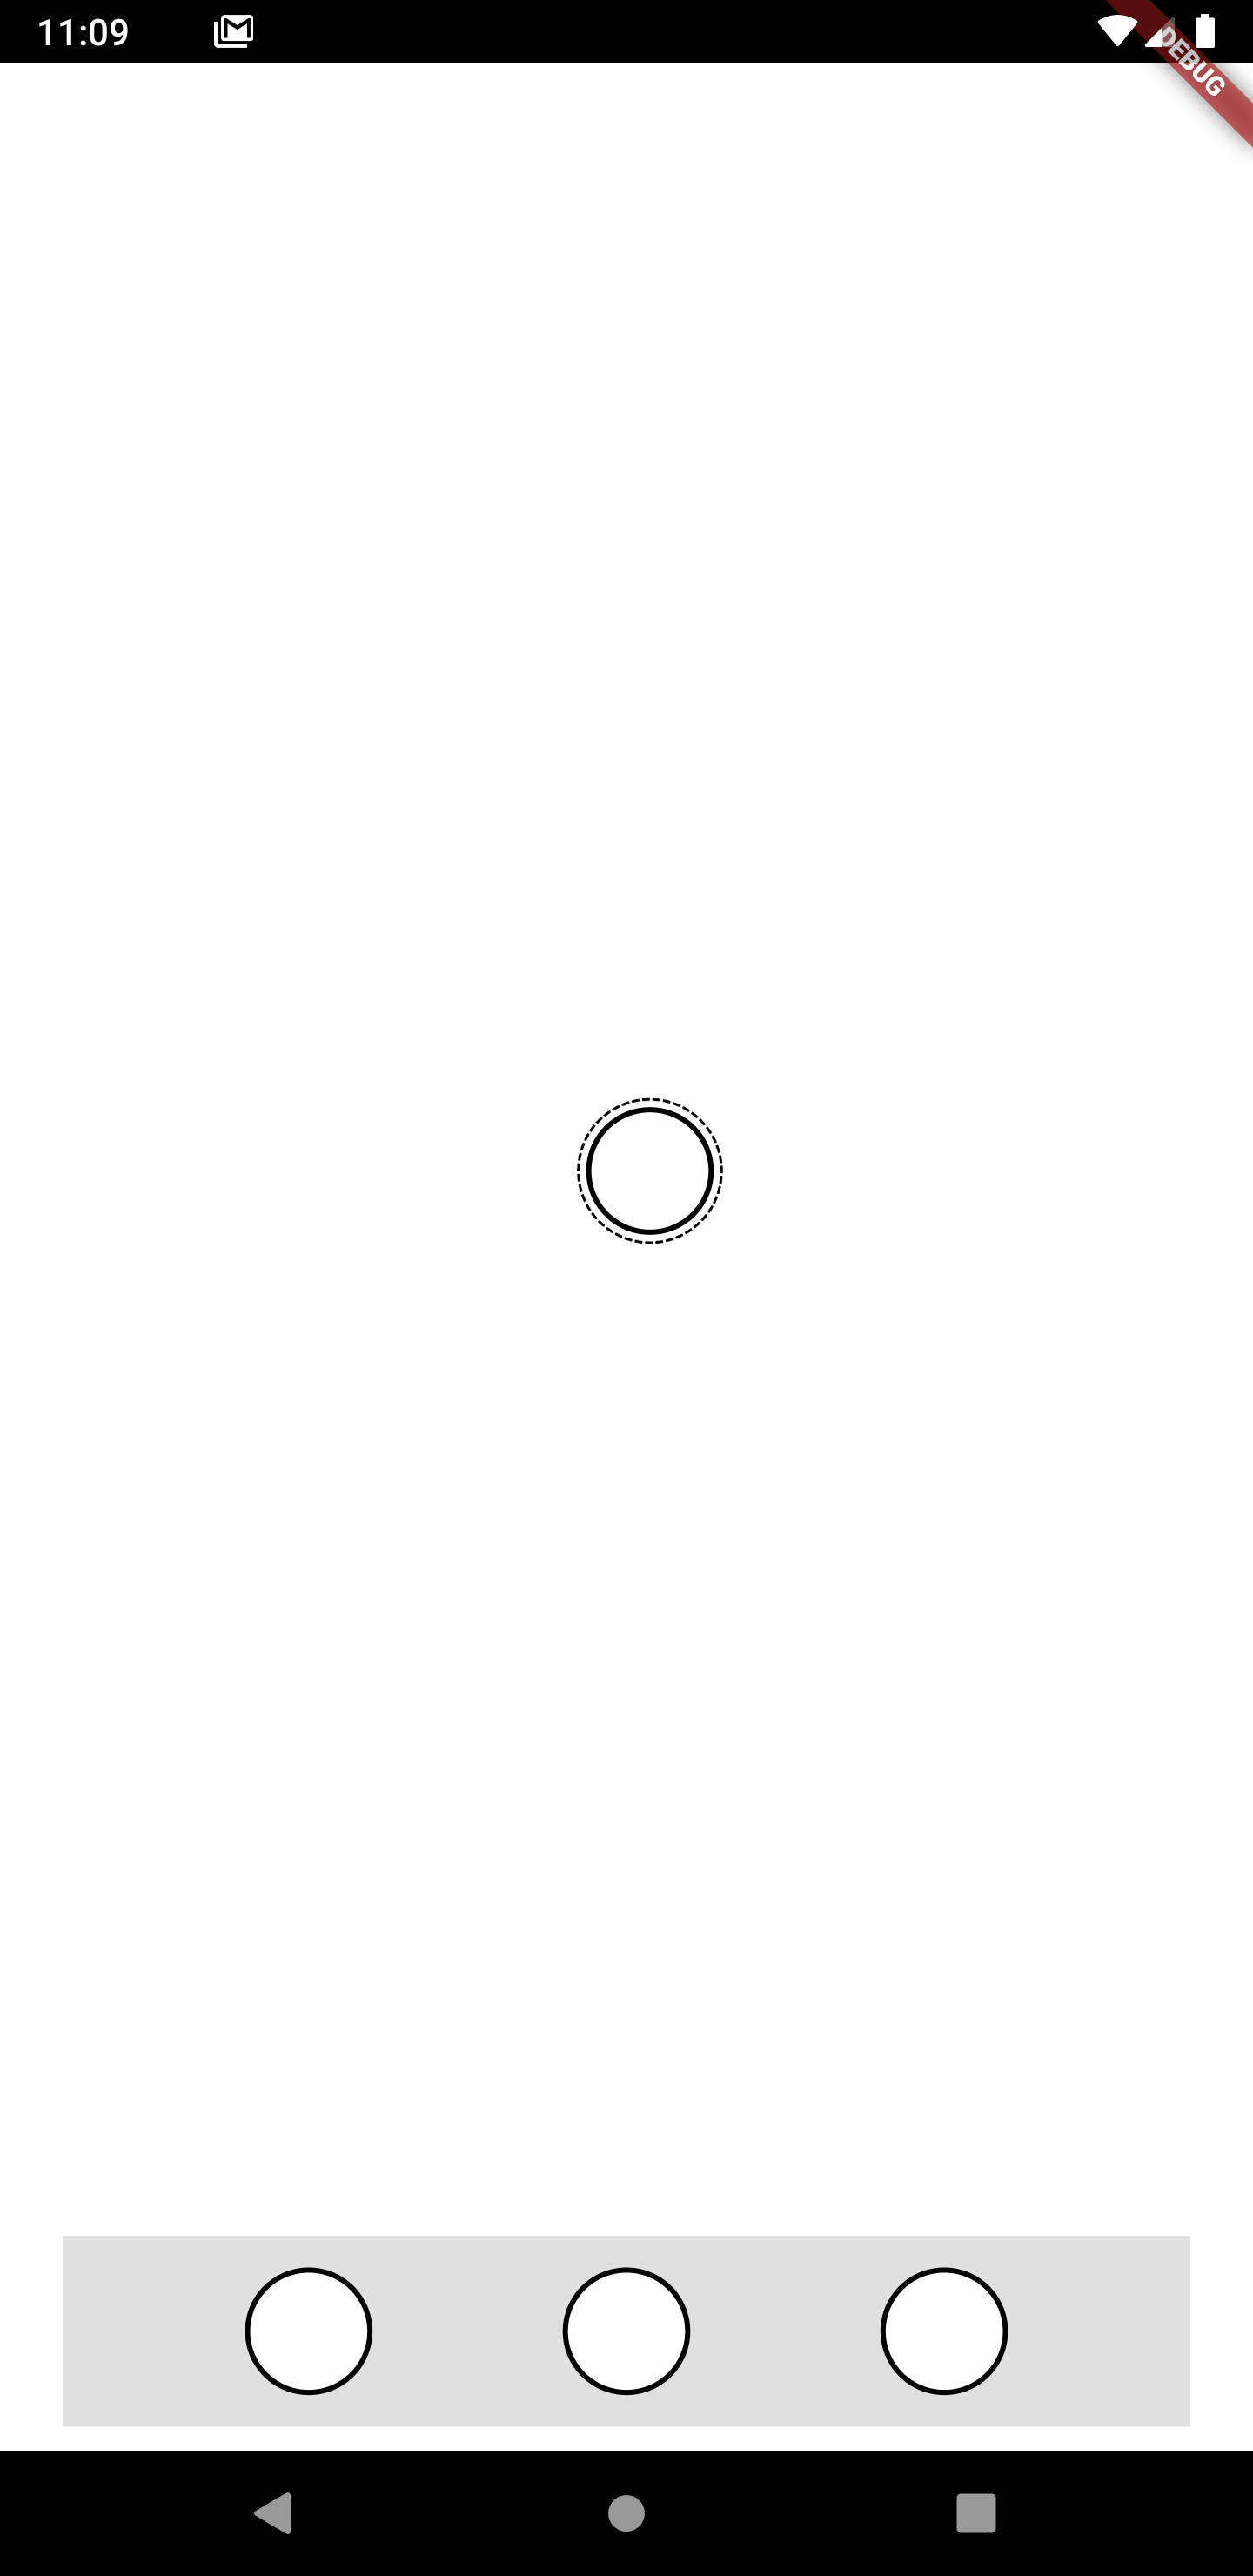
\includegraphics[width=5cm]{Images/App/zscale.png}
        \caption{Value c (3,3) = 2.0}
        \label{fig:zscaledemo}
    \end{subfigure}
    \hfill
    \begin{subfigure}{0.4\textwidth}
        \centering
        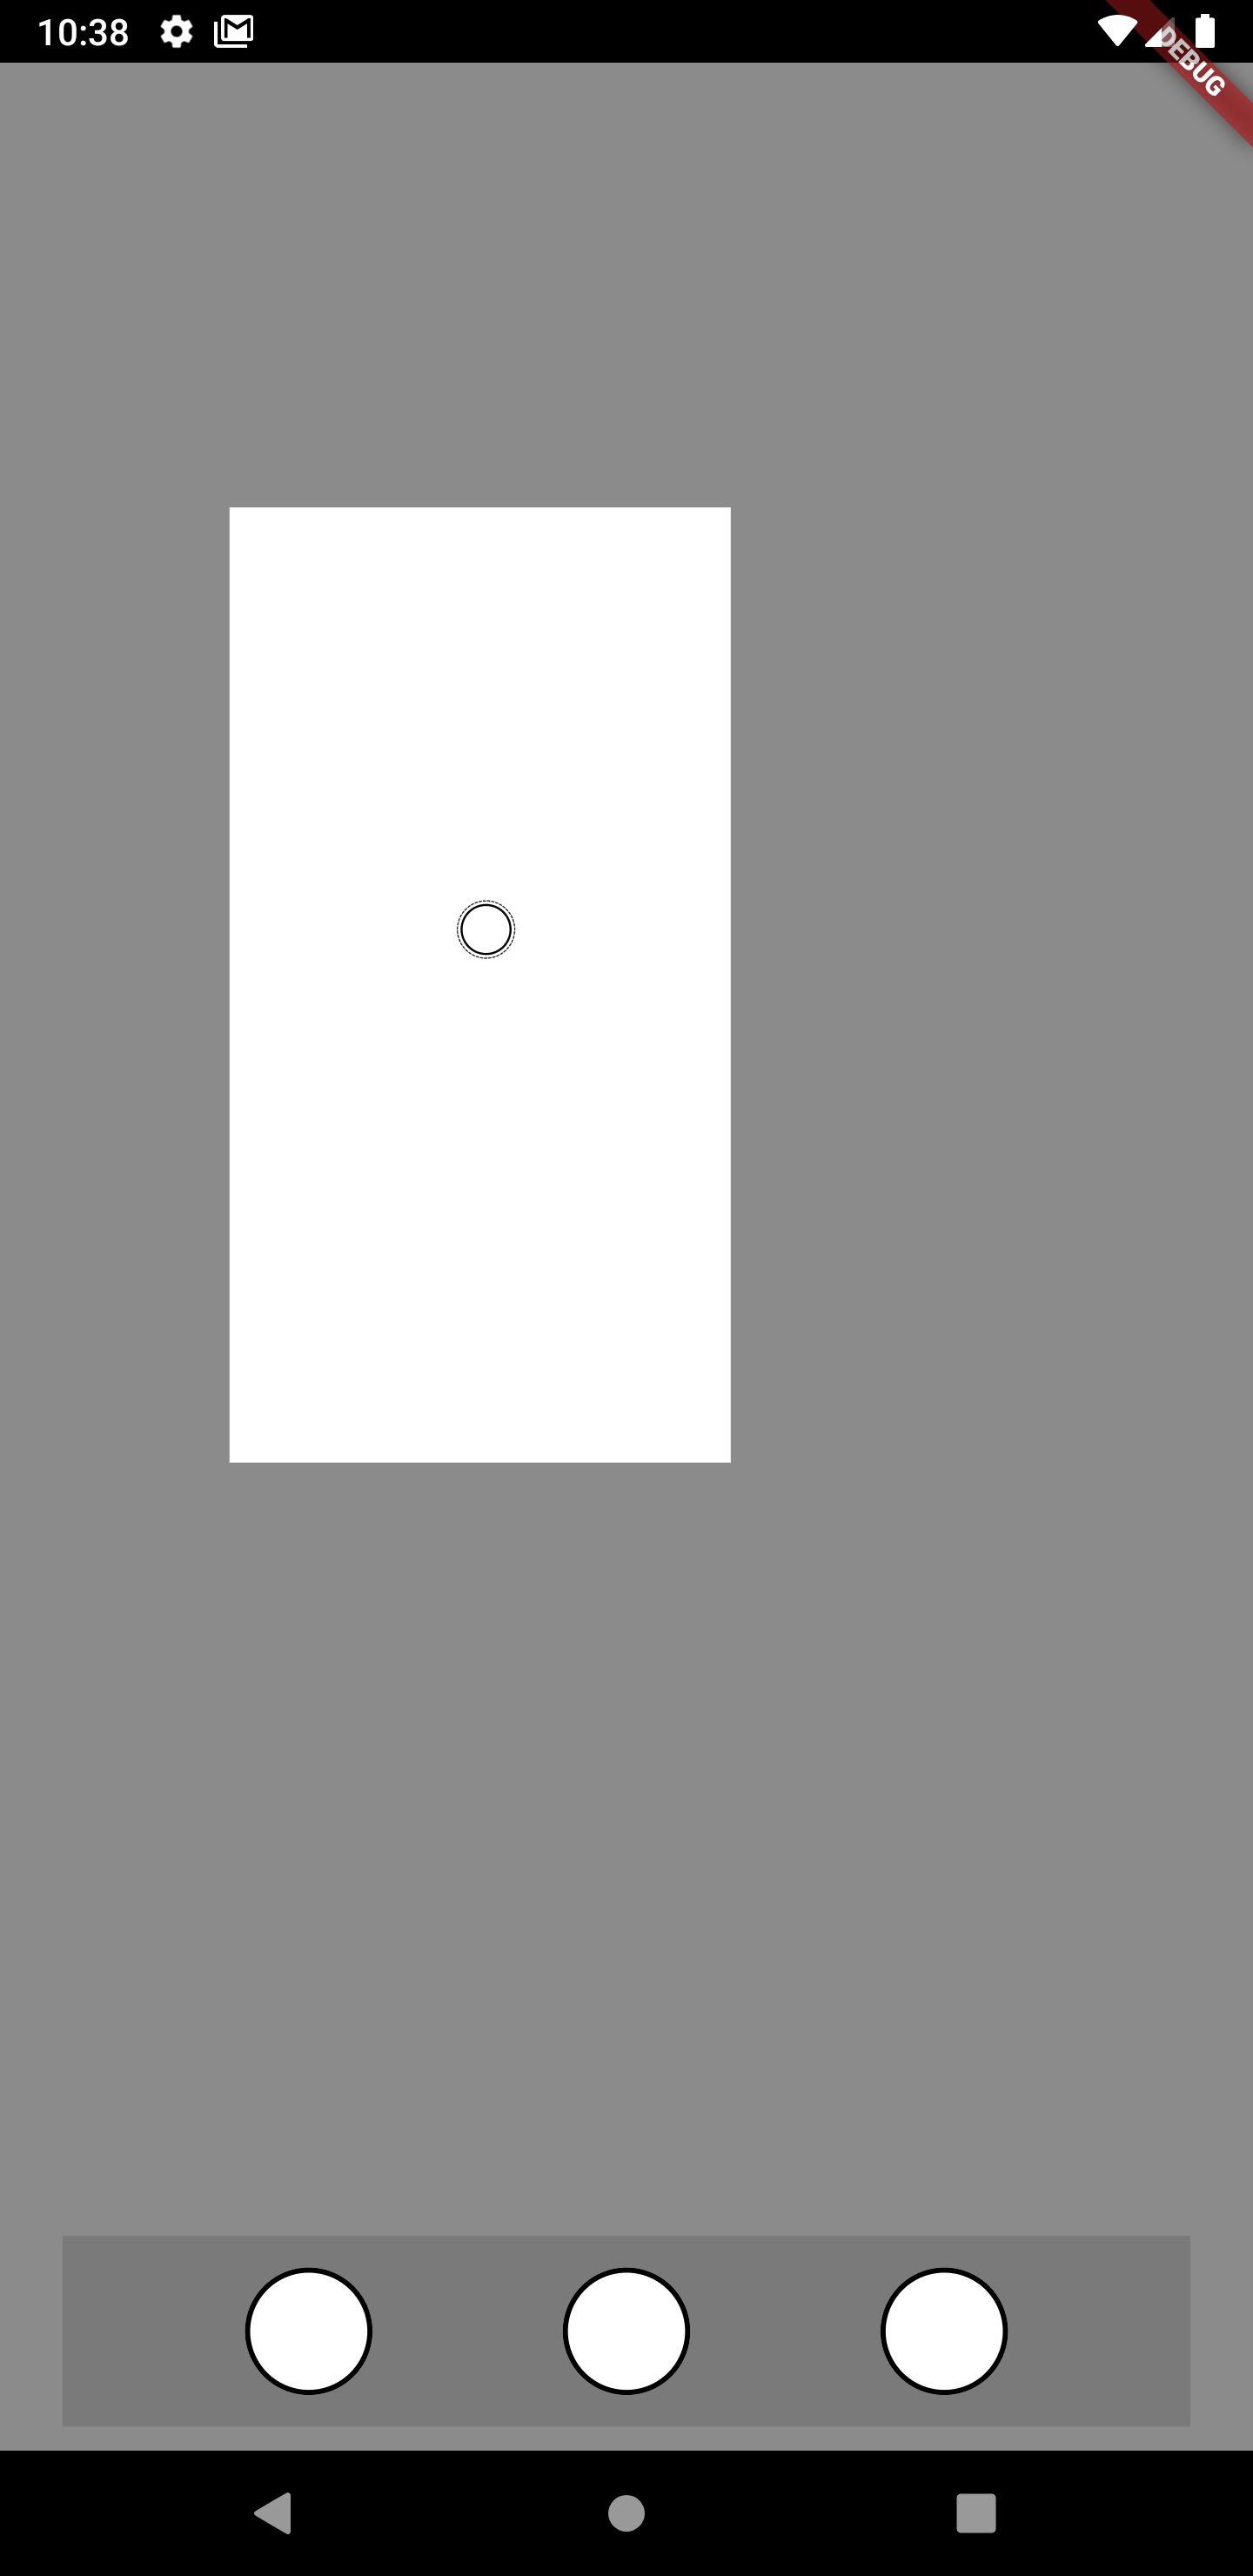
\includegraphics[width=5cm]{Images/App/zoomzscale.png}
        \caption{Zoom out with c = 2.0}
        \label{fig:zoomzscale}
    \end{subfigure}
    \caption{Scaling in Z}
    \label{fig:zscale}
\end{figure}

\begin{figure}[b]
    \begin{subfigure}{0.4\textwidth}
        \centering
        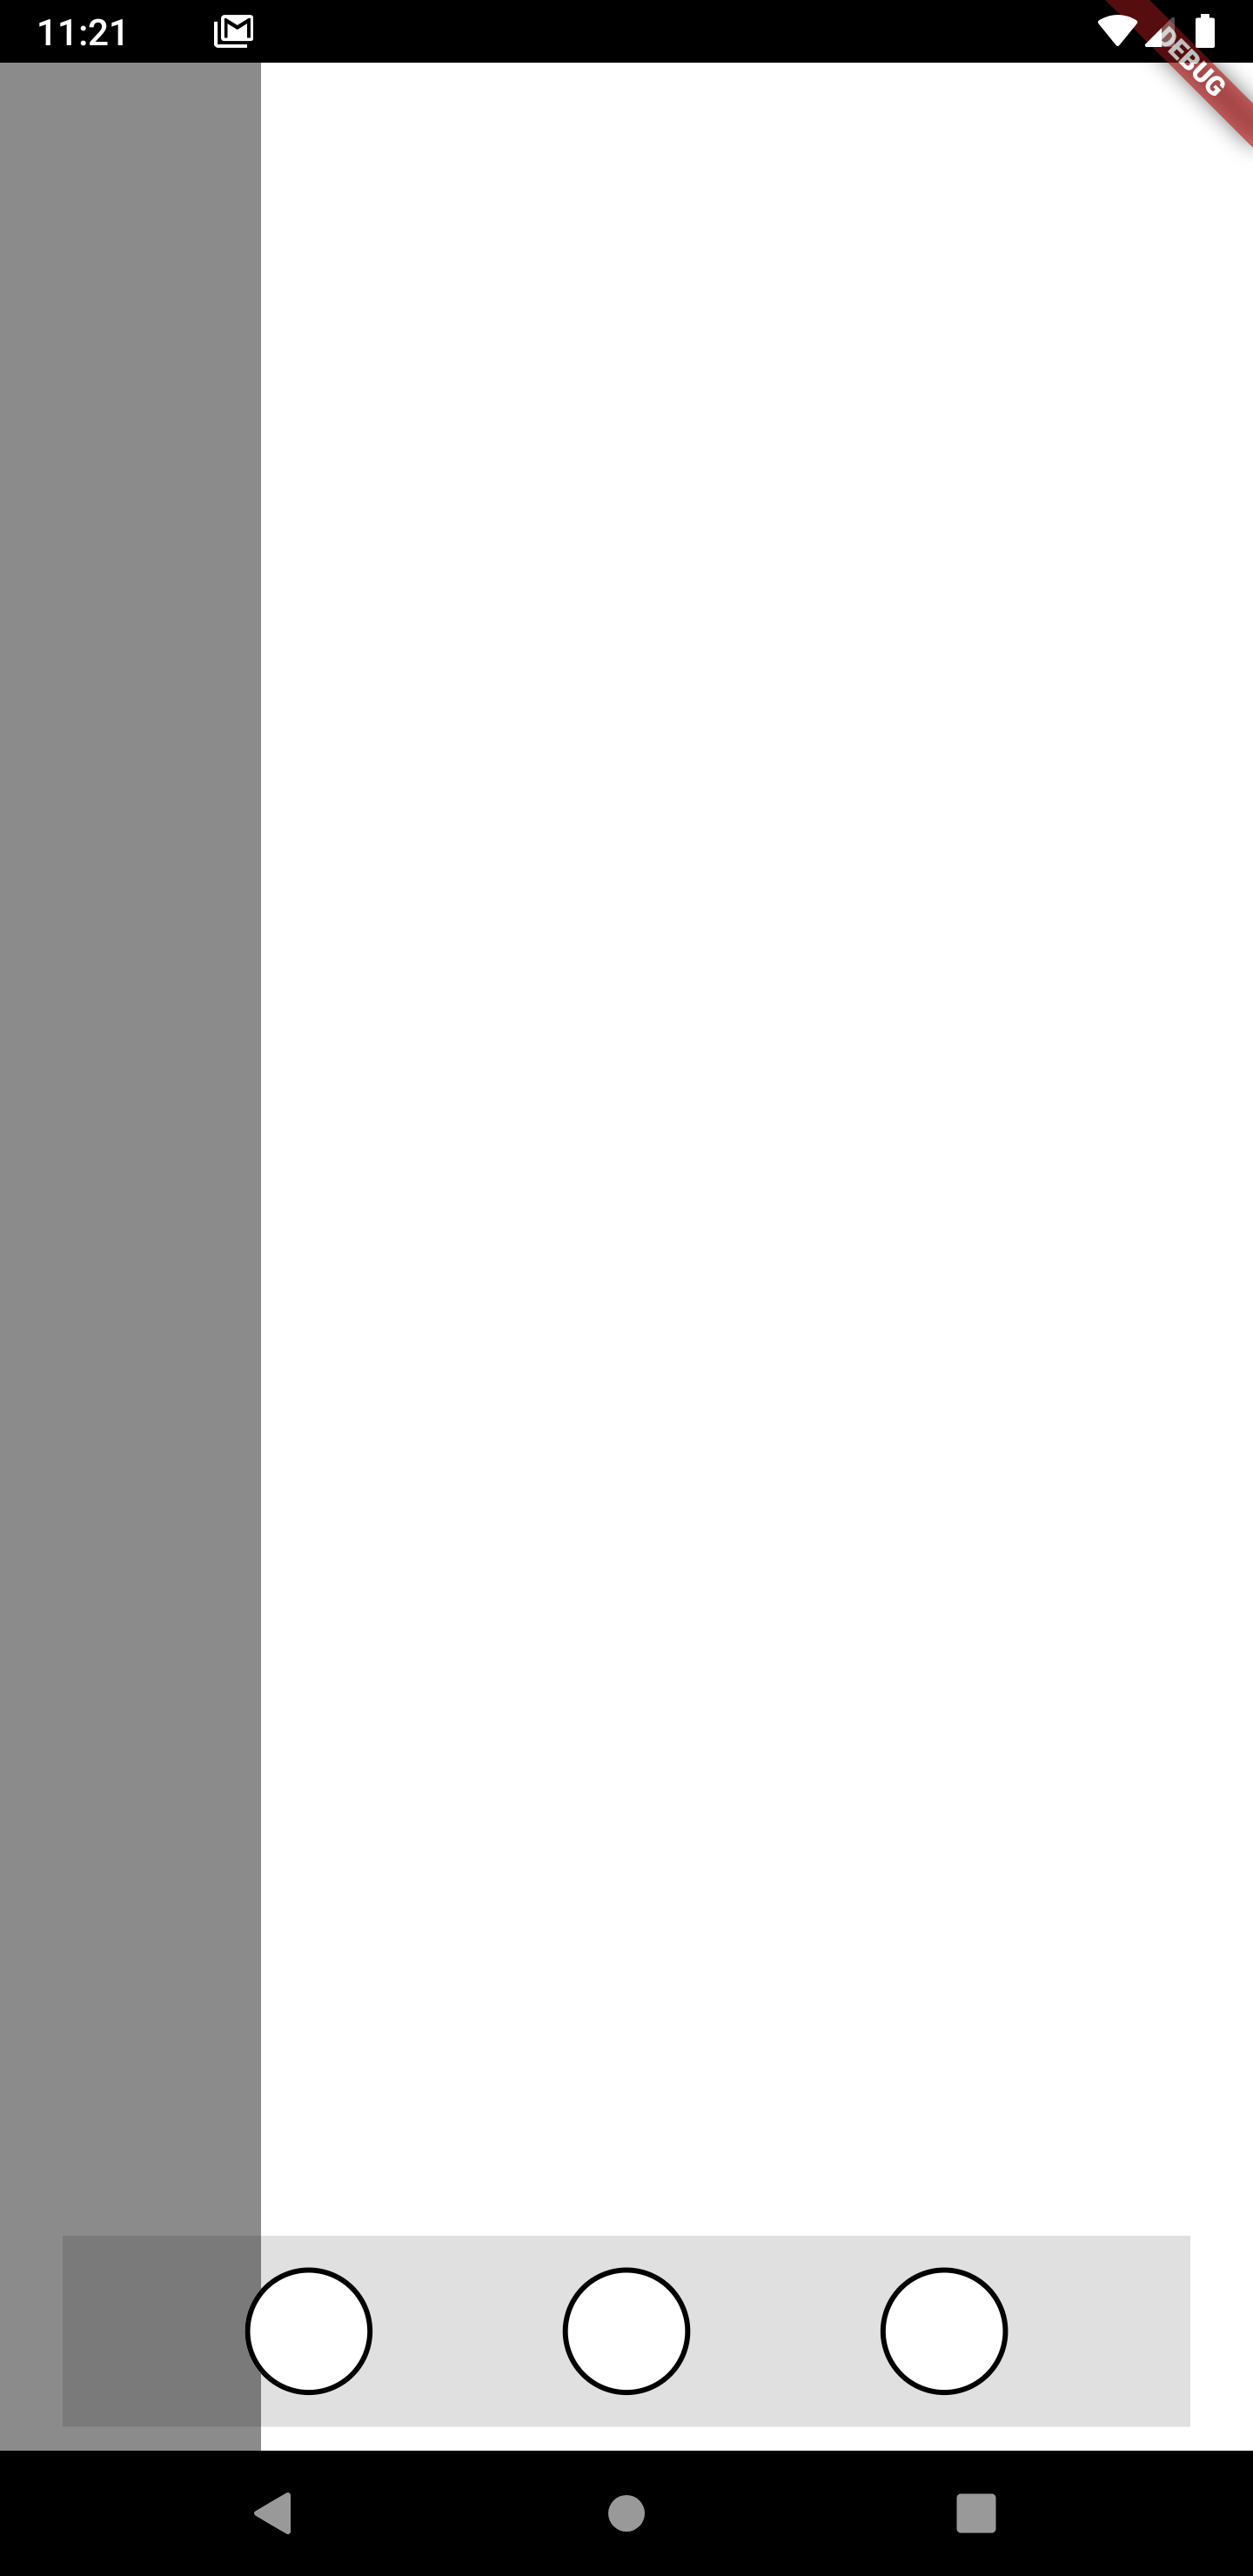
\includegraphics[width=5cm]{Images/App/xmove.png}
        \caption{Value d (4,1) = 100}
        \label{fig:xmove}
    \end{subfigure}
    \hfill
    \begin{subfigure}{0.4\textwidth}
        \centering
        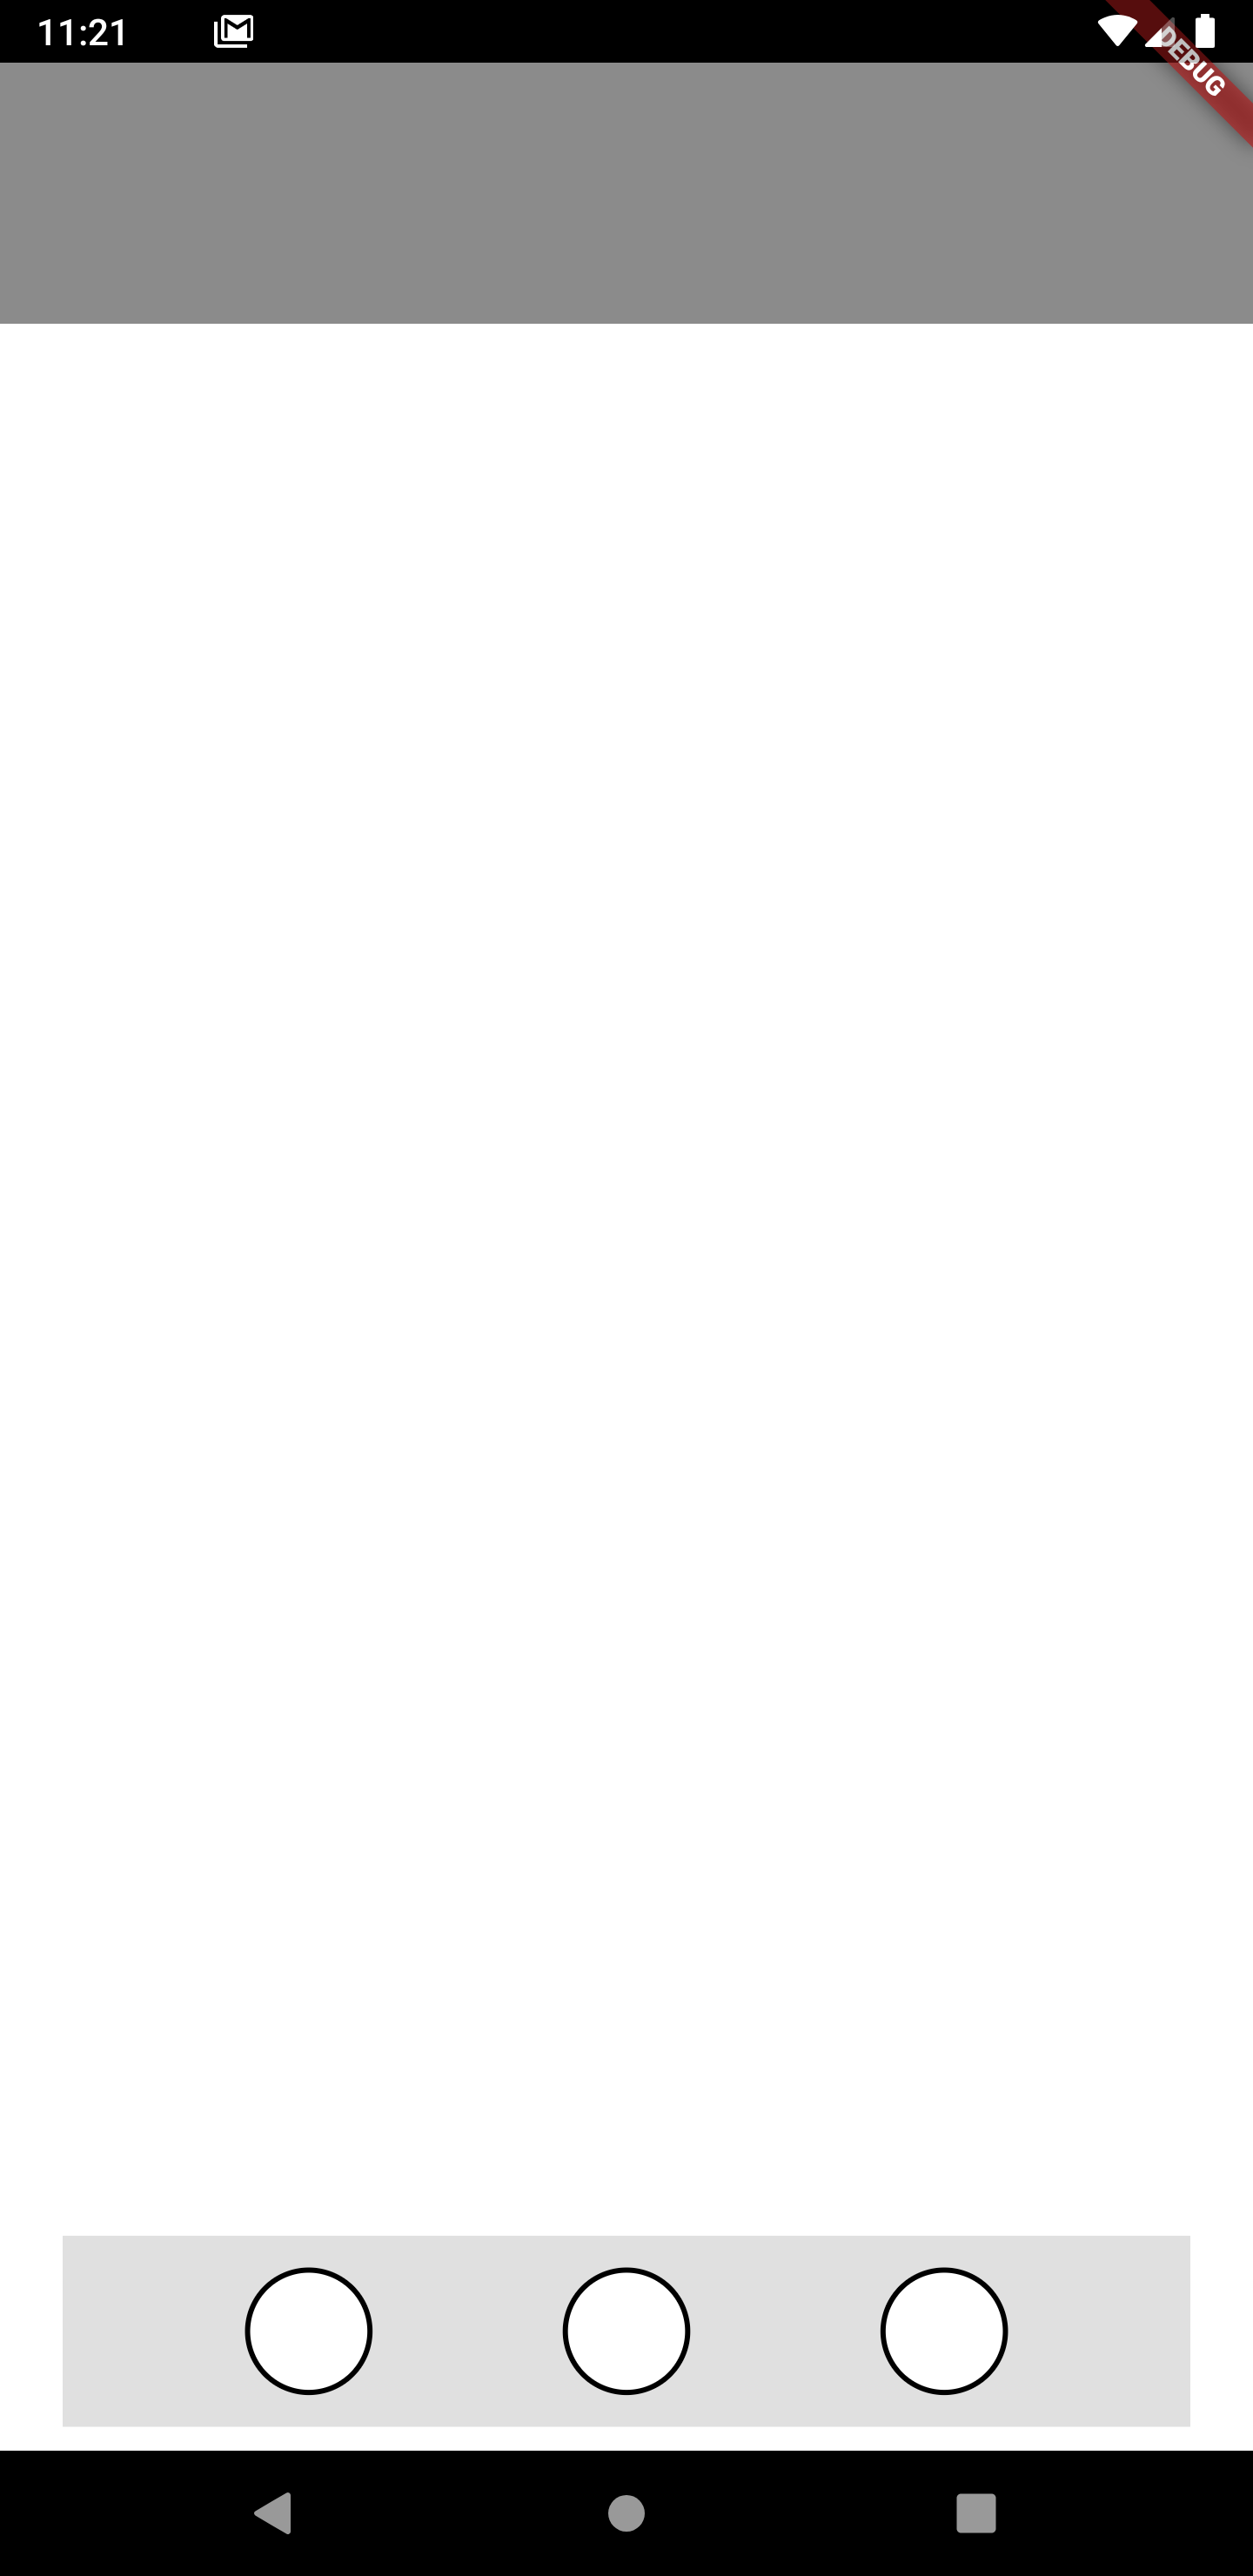
\includegraphics[width=5cm]{Images/App/ymove.png}
        \caption{Value e (4,2) = 100}
        \label{fig:ymove}
    \end{subfigure}
    \caption{Moving the space}
    \label{fig:moving}
\end{figure}

\begin{figure}[b]
    \begin{subfigure}{0.4\textwidth}
        \centering
        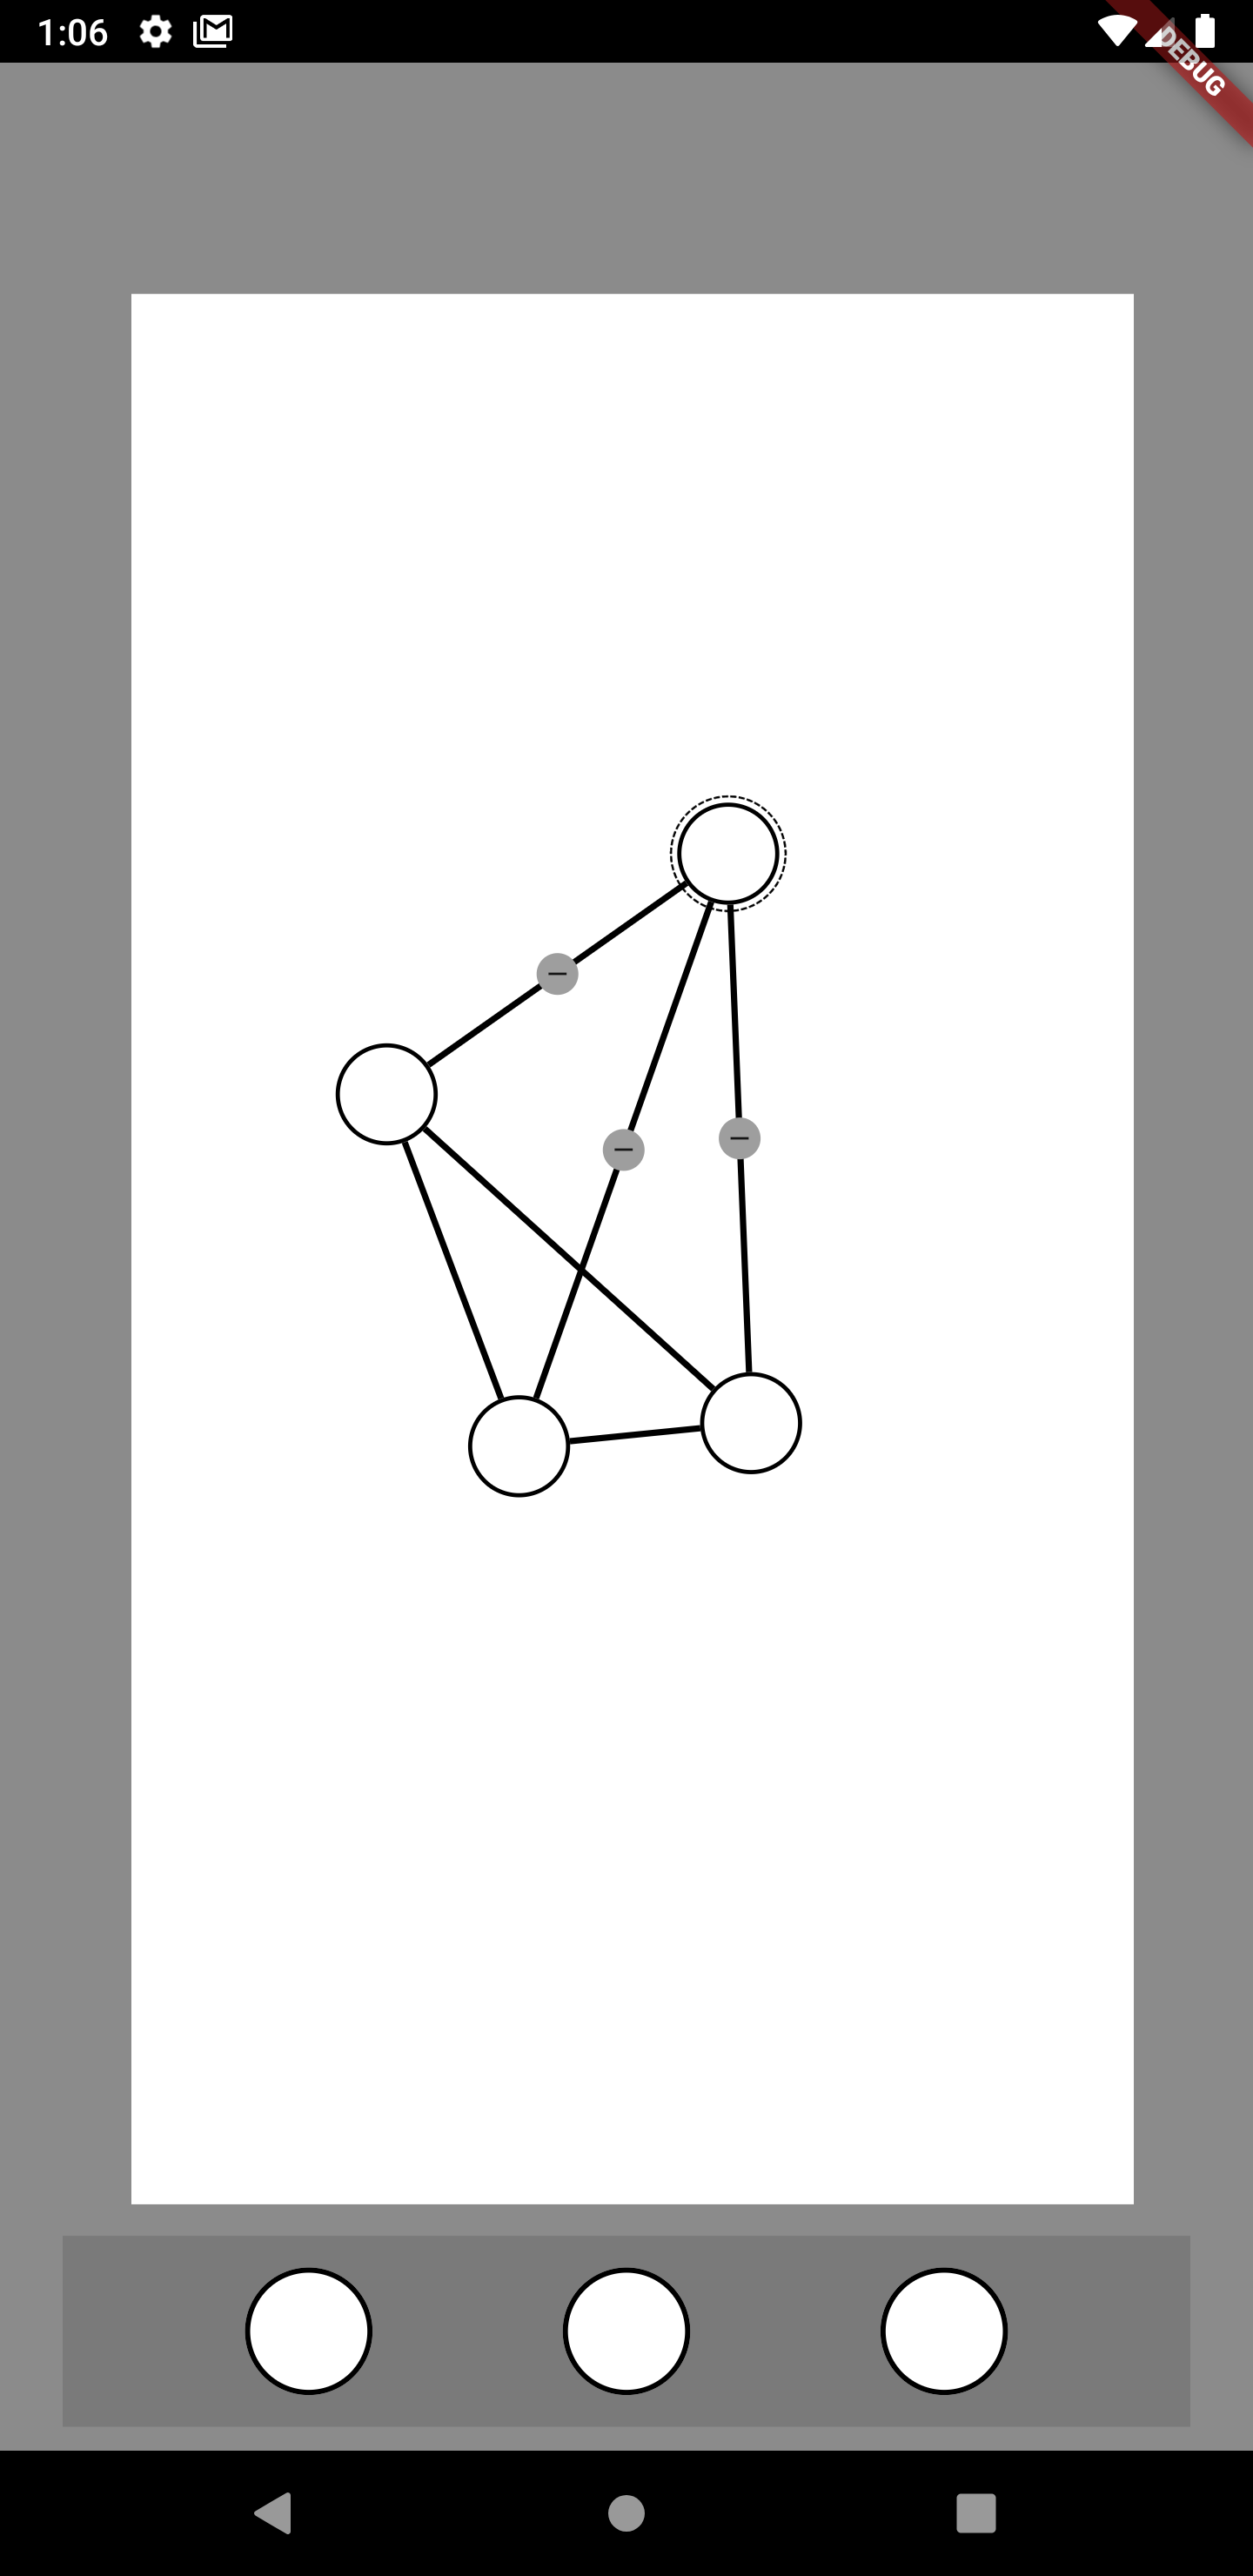
\includegraphics[width=4cm]{Images/App/AppDemo1.png}
        \label{fig:demo1}
    \end{subfigure}
    \hfill
    \begin{subfigure}{0.4\textwidth}
        \centering
        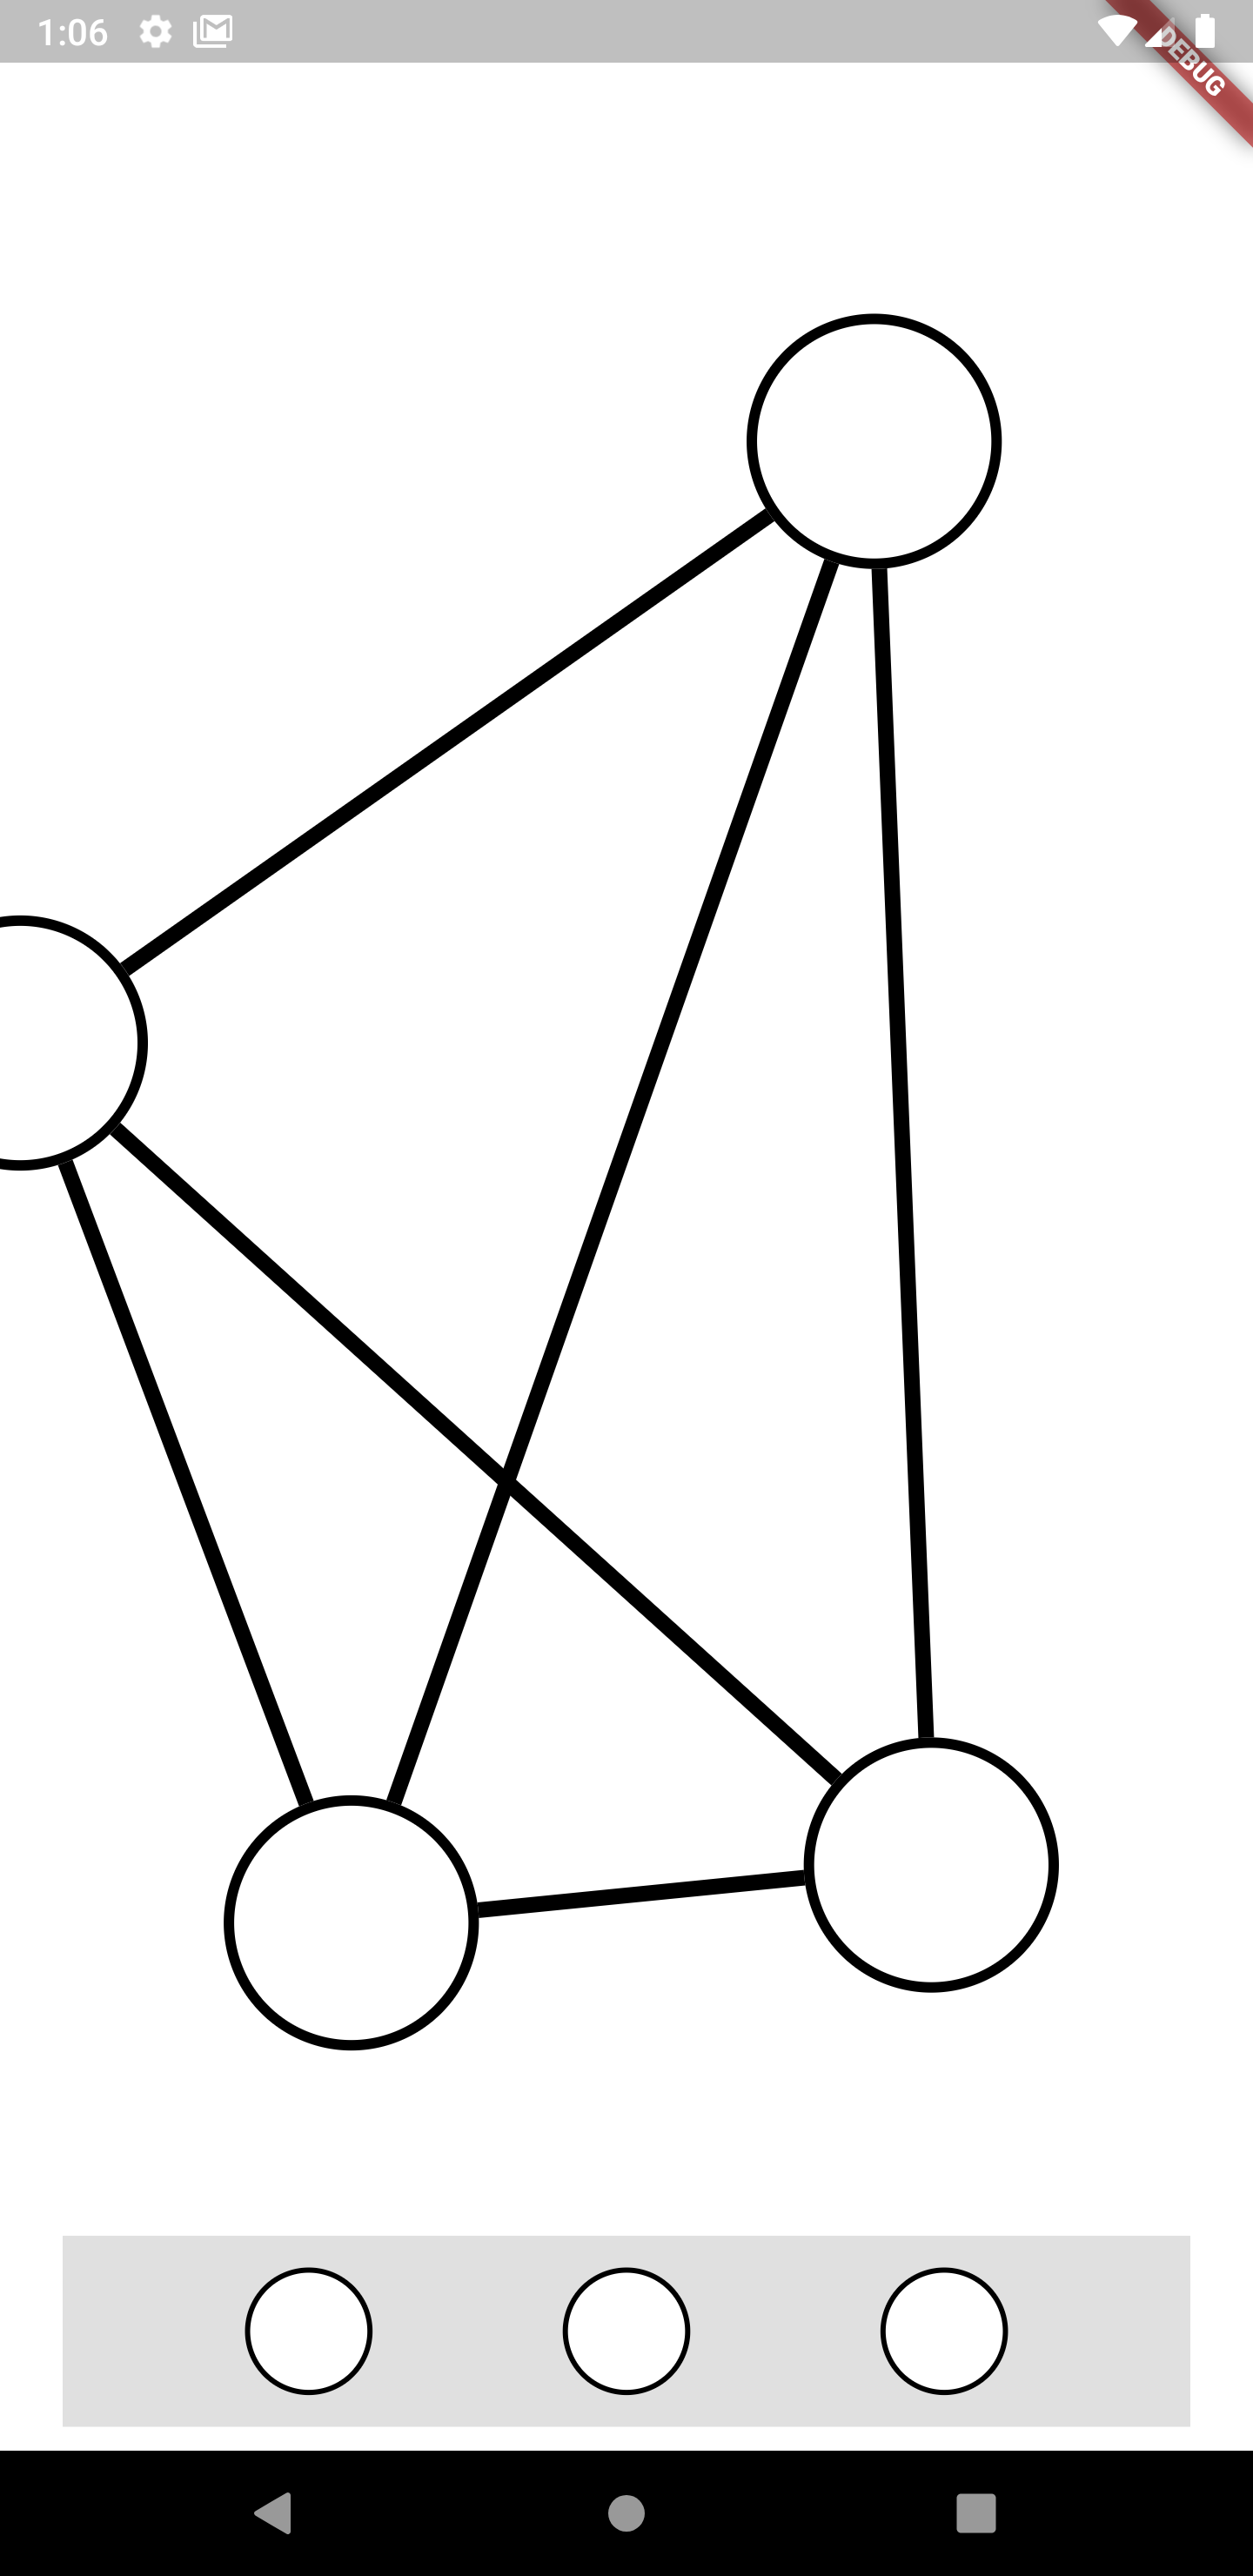
\includegraphics[width=4cm]{Images/App/AppDemo2.png}
        \label{fig:demo2}
    \end{subfigure}
    \caption{Diagram display result}
    \label{fig:result}
\end{figure}

